\documentclass[12pt,a4paper]{article}

% ========================
% PACKAGES
% ========================
\usepackage[utf8]{vietnam}
\usepackage[T5]{fontenc}
\usepackage[hidelinks]{hyperref}
\usepackage{xurl}
\usepackage{graphicx}
\usepackage{fancyhdr}
\usepackage{geometry}
\usepackage{titlesec}
\usepackage{color}
\usepackage{framed}
\usepackage{longtable}
\usepackage{amsmath, amssymb}
\usepackage{caption}
\usepackage{subcaption}
\usepackage{booktabs}
\usepackage{tikz}
\usepackage{float}
\usepackage{graphicx}
\usetikzlibrary{calc} % Thư viện để tính toán toạ độ cho khung viền

% ========================
% PAGE SETUP
% ========================
\geometry{
  a4paper,
  left=2.5cm,
  right=2.5cm,
  top=2.5cm,
  bottom=2.5cm,
  headheight=15pt
}

\pagestyle{fancy}
\fancyhf{}
\fancyhead[L]{IE207 Đồ án}
\fancyhead[R]{Federated Learning}
\fancyfoot[C]{\thepage}

% ========================
% NUMBERING CONFIG
% ========================
\setcounter{secnumdepth}{3} 
\setcounter{tocdepth}{3}

\renewcommand{\thesection}{\Roman{section}}
\renewcommand{\thesubsection}{\arabic{subsection}}
\renewcommand{\thesubsubsection}{\thesubsection.\arabic{subsubsection}}

% ========================
% TITLE FORMAT
% ========================
\titleformat{\section}[block]
  {\normalfont\Large\bfseries\centering}
  {CHƯƠNG \thesection:}
  {0.5em}
  {\MakeUppercase}

\titleformat{\subsection}
  {\normalfont\large\bfseries}
  {\thesubsection.}
  {0.5em}
  {}

\titleformat{\subsubsection}
  {\normalfont\normalsize\bfseries}
  {\thesubsubsection.}
  {0.5em}
  {}

% ========================
% DOCUMENT
% ========================
\begin{document}

% ========================
% TITLE PAGE
% ========================
\begin{titlepage}
    % --- TẠO KHUNG VIỀN (Giữ nguyên) ---
    \begin{tikzpicture}[overlay,remember picture]
        \draw [line width=3pt]
            ($ (current page.north west) + (2.0cm,-2.0cm) $)
            rectangle
            ($ (current page.south east) + (-2.0cm,2.0cm) $);
        \draw [line width=1pt]
            ($ (current page.north west) + (2.15cm,-2.15cm) $)
            rectangle
            ($ (current page.south east) + (-2.15cm,2.15cm) $); 
    \end{tikzpicture}

    \begin{center}
        \vspace*{-0.5cm} % Kéo nội dung lên cao một chút để tránh tràn dưới
        
        % --- HEADER ---
        \textbf{\large ĐẠI HỌC QUỐC GIA TP. HỒ CHÍ MINH} \\
        \textbf{\large TRƯỜNG ĐẠI HỌC CÔNG NGHỆ THÔNG TIN} \\
        \textbf{\large KHOA KHOA HỌC VÀ KỸ THUẬT THÔNG TIN} \\
        
        \vspace{1cm} % Khoảng cách đến Logo

        % --- LOGO ---
        % Giảm kích thước logo xuống xíu cho đỡ chiếm chỗ (4cm -> 3.5cm)
        
\includegraphics[width=3.5cm]{asset/uit_logo.png} 
        
        \vspace{1cm} % Khoảng cách đến tên Báo cáo

        % --- REPORT TYPE ---
        \textbf{\LARGE BÁO CÁO ĐỒ ÁN} \\[0.3cm]
        \textbf{\Large Môn: IE207 Đồ án} \\
        
        \vspace{1.5cm} % Khoảng cách đến Tên đề tài

        % --- TITLE ---
        \textbf{\Large ĐỀ TÀI:} \\[0.3cm]
        \begin{minipage}{0.9\textwidth}
            \centering
            % Dùng \parbox hoặc để tự nhiên, LaTeX sẽ tự xuống dòng nếu tên quá dài
            \textbf{\MakeUppercase{Nghiên cứu các mô hình trong Học Liên Kết (Federated Learning) sử dụng Flower framework}}
        \end{minipage}
        
        \vfill % Tự động đẩy phần thông tin xuống dưới, nhưng không quá sát đáy

        % --- INFO TABLE (Đã sửa lại form cho nhóm) ---
        \begin{table}[h]
            \centering
            \renewcommand{\arraystretch}{1.2} % Tăng khoảng cách giữa các dòng trong bảng cho dễ nhìn
            \begin{tabular}{p{5cm} l} % Cột 1 rộng 5cm, Cột 2 tự động dãn
                \textbf{Giảng viên hướng dẫn:} & TS. Nguyễn Tấn Cầm \\
                & \\ % Dòng trống tạo khoảng cách
                \textbf{Sinh viên thực hiện:}  & 1. Trần Tấn Khải - 23520680 \\ % Tên 1
                                               & 2. Trần Hải Đông - 23520300 \\   % Tên 2
                & \\ % Dòng trống
                \textbf{Lớp:}                  & IE207.Q11.CNVN
            \end{tabular}
        \end{table}

        \vfill % Đẩy ngày tháng xuống sát khung dưới
        
        % --- DATE ---
        \textbf{TP. Hồ Chí Minh, tháng 12 năm 2025}
        \vspace{1cm} % Tạo khoảng hở nhỏ so với khung viền dưới
    \end{center}
\end{titlepage}

% ==================================================================
% TRANG 1: DANH SÁCH THÀNH VIÊN & PHÂN CÔNG (Ảnh thẻ DỌC)
% ==================================================================
\begin{center}
     \textbf{\Large DANH SÁCH THÀNH VIÊN NHÓM}
\end{center}
\vspace{0.2cm} % Tạo một chút khoảng cách với hình bên dưới
\begin{figure}[h]
    \centering
    % --- THÀNH VIÊN 1 ---
    \begin{minipage}{0.25\textwidth}
        \centering
        \begin{tikzpicture}
            % 1. Vẽ khung viền (để hiển thị)
            \draw[thick] (0,0) rectangle (3,4);
            
            % 2. Tạo vùng cắt ảnh (clipping path)
            % Bất cứ thứ gì vẽ sau dòng này sẽ chỉ hiển thị trong hình chữ nhật này.
            \clip (0,0) rectangle (3,4);
            
            % 3. Chèn ảnh và căn giữa vùng cắt
            % width=3cm: Đặt chiều rộng ảnh là 3cm để vừa chiều ngang khung.
            % keepaspectratio: Giữ nguyên tỉ lệ ảnh, chiều cao tự động điều chỉnh.
            % at (1.5,2): Đặt tâm ảnh vào tâm của khung cắt.
            % Thay đường dẫn ảnh thực tế của bạn vào đây: {asset/chien.jpg}
            \node at (1.5,2) {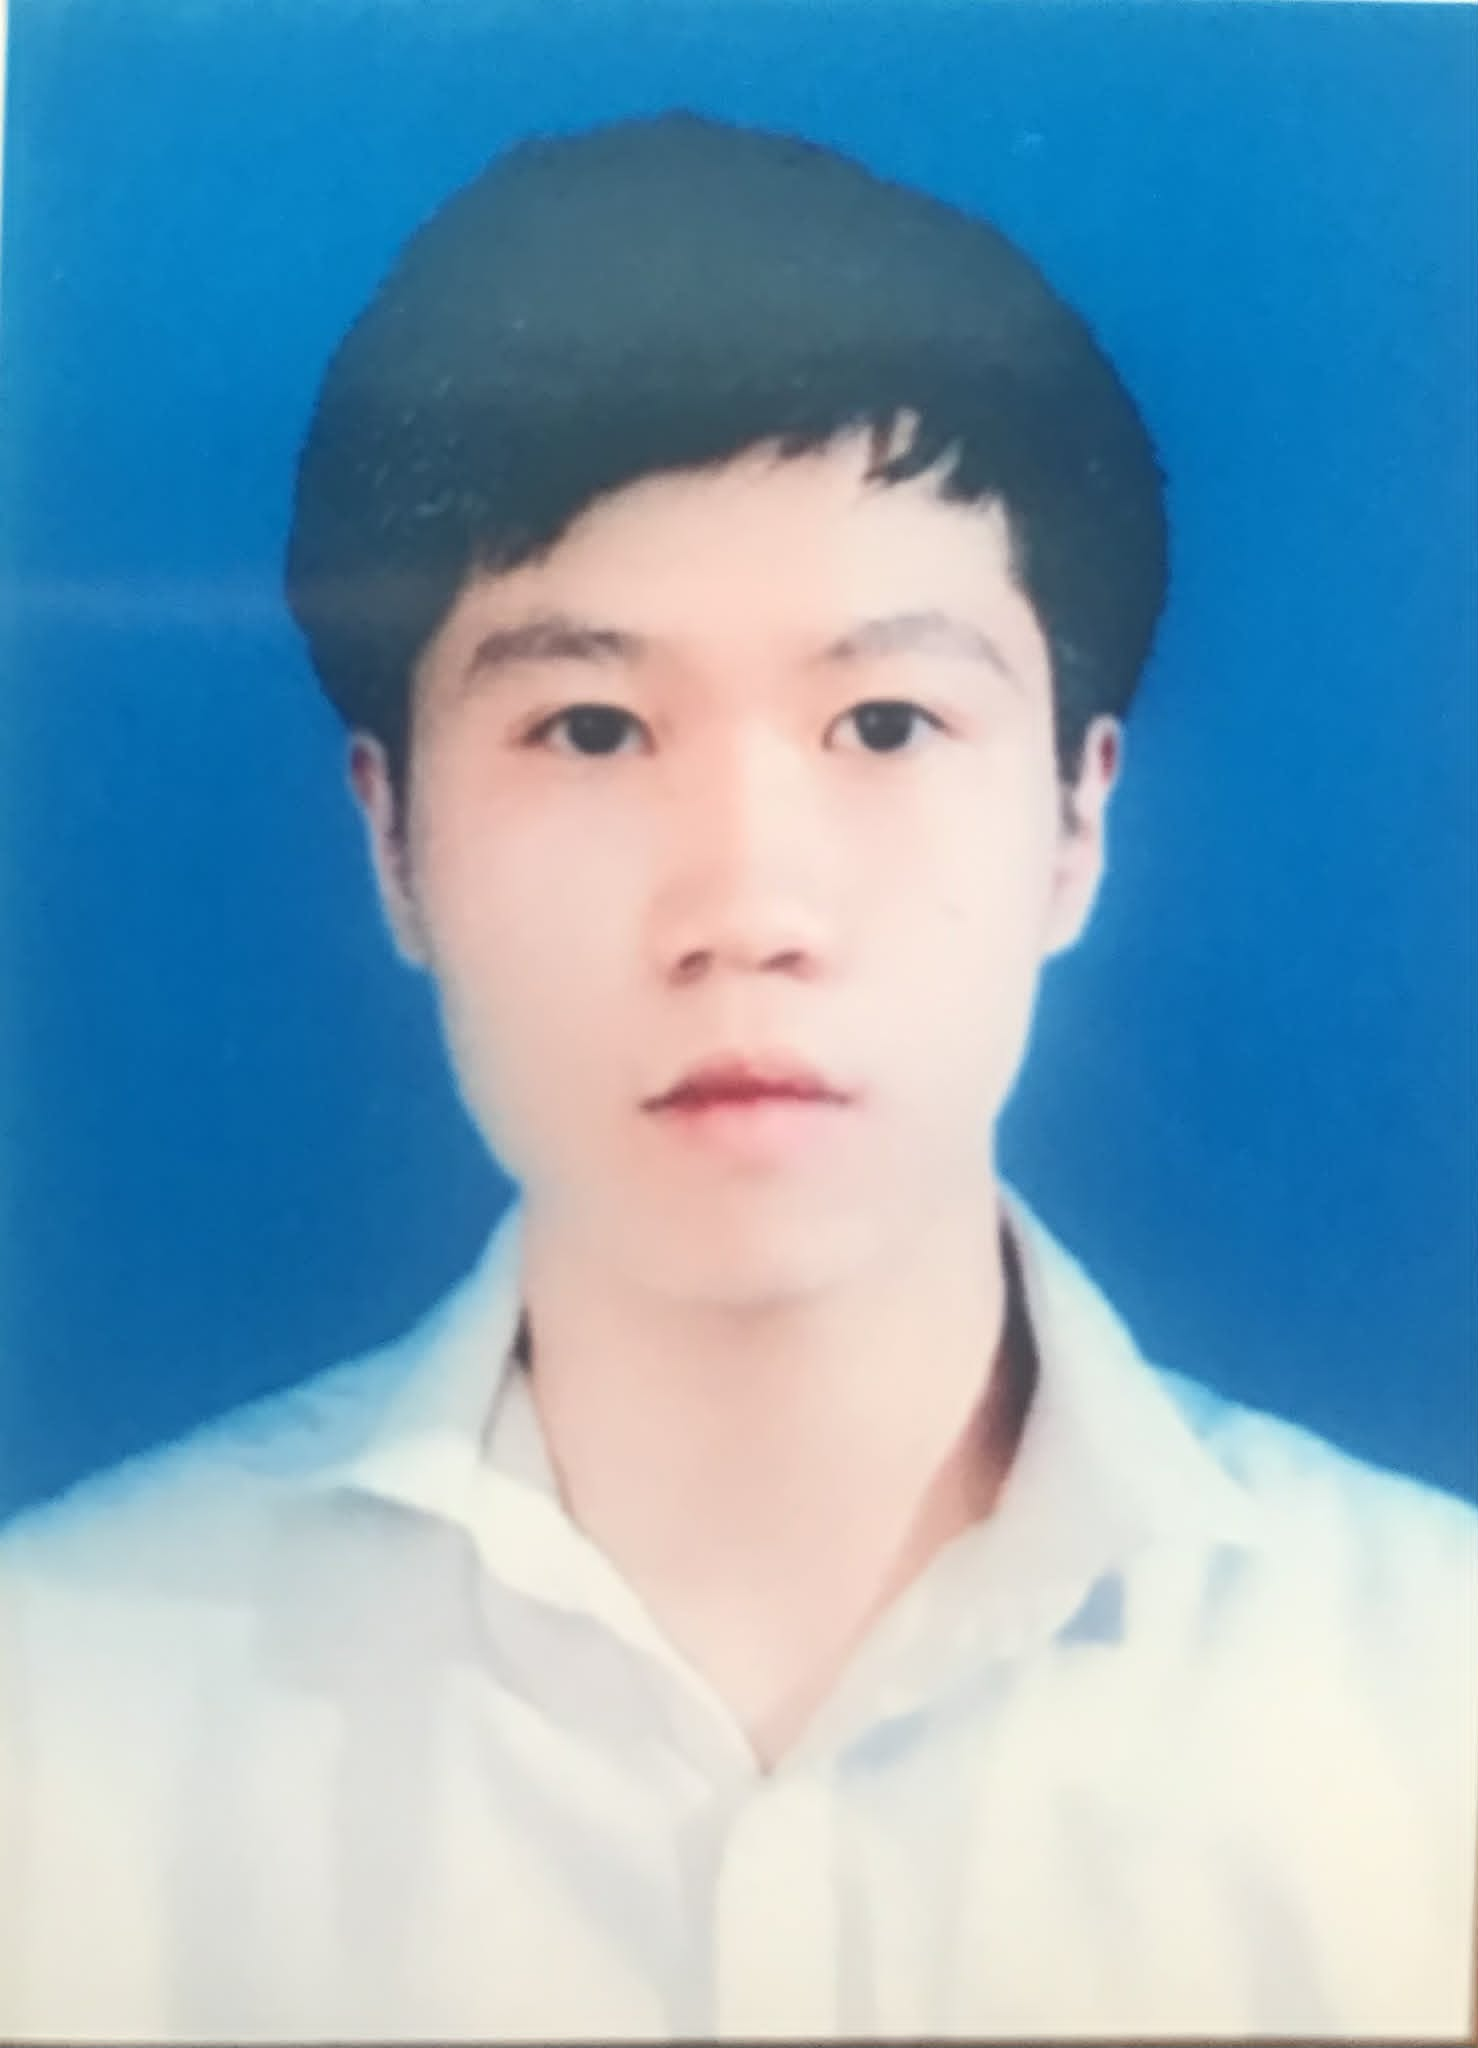
\includegraphics[width=3cm, keepaspectratio]{asset/download (1).jpeg}};
        \end{tikzpicture}
        \vspace{0.3cm}
        
        \textbf{Trần Tấn Khải}\\
        MSSV: 23520680\\
        (Nhóm trưởng)
    \end{minipage}
    \hfill
    % --- THÀNH VIÊN 2 ---
    \begin{minipage}{0.25\textwidth}
        \centering
        \begin{tikzpicture}
            \draw[thick] (0,0) rectangle (3,4);
            \clip (0,0) rectangle (3,4);
            \node at (1.5,2) {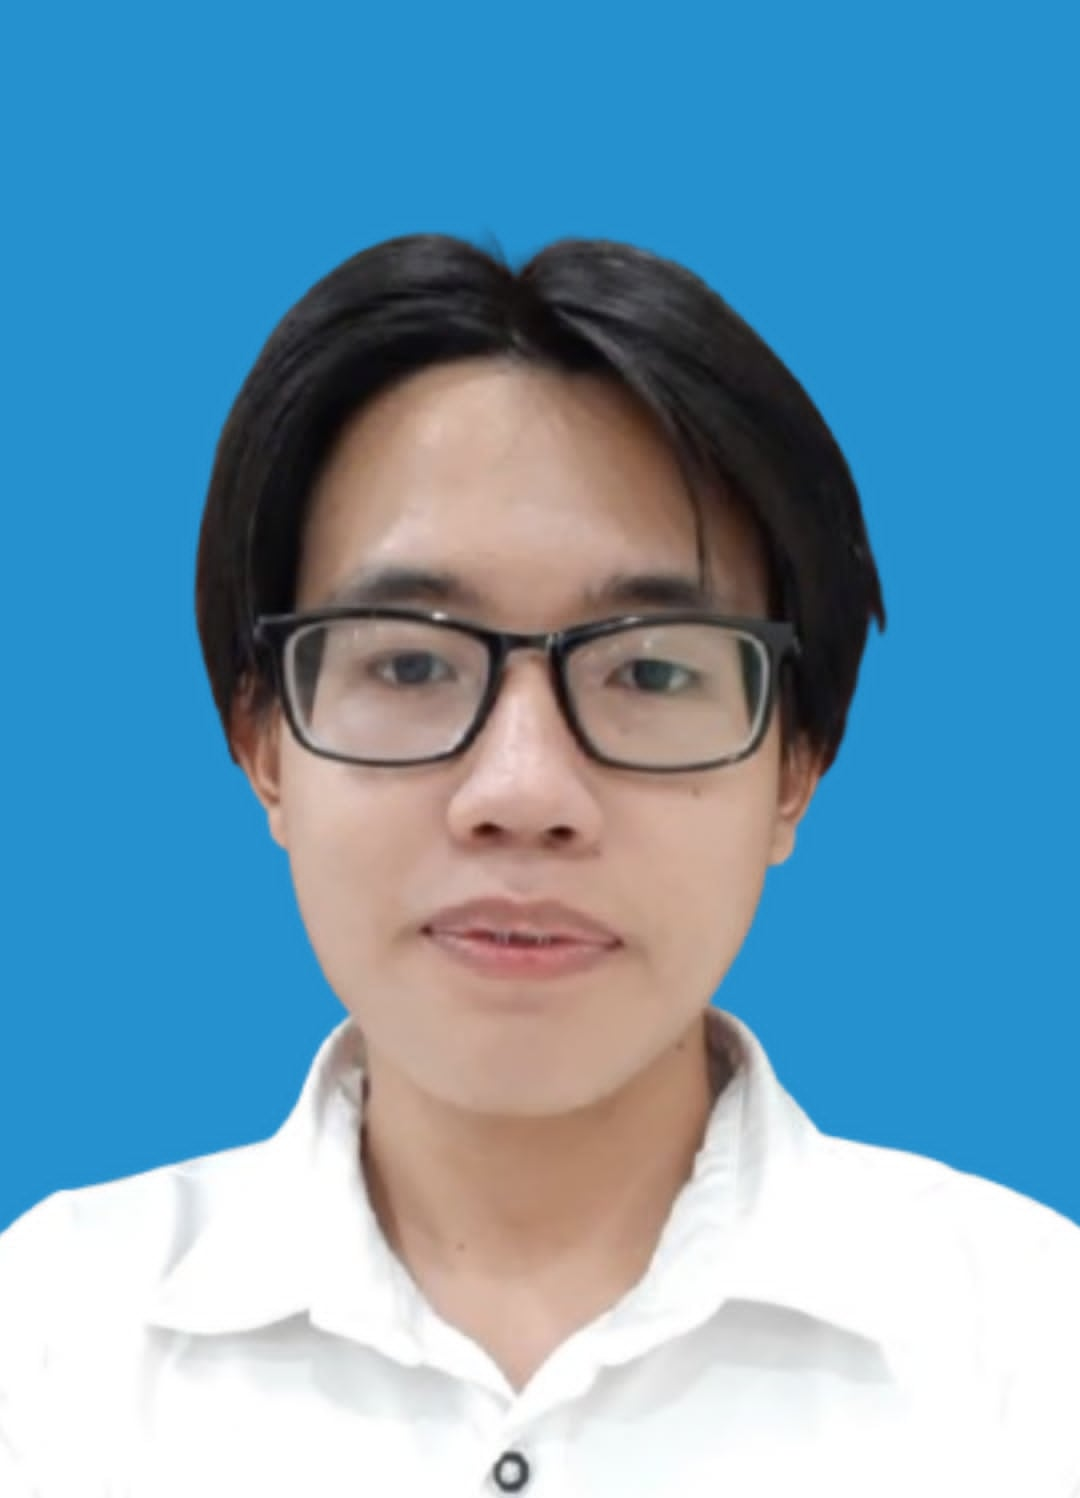
\includegraphics[width=3cm, keepaspectratio]{asset/download.jpeg}};
        \end{tikzpicture}
        \vspace{0.3cm}
        
        \textbf{Trần Hải Đông}\\
        MSSV: 23520300\\
        (Thành viên)
    \end{minipage}
\end{figure}

\vspace{0.5cm}


% ==================================================================
% LỜI CẢM ƠN
% ==================================================================
\newpage
\thispagestyle{empty} % Không đánh số trang cho trang này

\begin{center}
    \section*{LỜI CẢM ƠN}
    \addcontentsline{toc}{section}{Lời cảm ơn} % Thêm vào mục lục dù không đánh số chương
\end{center}

\vspace{1cm}

Lời đầu tiên, chúng em xin gửi lời cảm ơn chân thành và sâu sắc nhất đến TS. Nguyễn Tấn Cầm, giảng viên hướng dẫn môn học IE207 Đồ án. Thầy đã tận tình truyền đạt những kiến thức nền tảng quý báu, định hướng tư duy nghiên cứu và tạo mọi điều kiện thuận lợi để chúng em có thể tiếp cận với đề tài đầy thách thức nhưng cũng rất thú vị về \textit{Federated Learning} sử dụng \textit{Flower framework}.

Chúng em cũng xin gửi lời tri ân đến quý Thầy, Cô trong Khoa Khoa học và Kỹ thuật Thông tin cùng Ban Giám hiệu Trường Đại học Công nghệ Thông tin (ĐHQG-HCM) đã xây dựng môi trường học tập năng động, sáng tạo và cung cấp cơ sở vật chất tốt nhất để sinh viên chúng em có thể hoàn thành đồ án này.

Đặc biệt, đồ án này là kết quả của sự nỗ lực không ngừng nghỉ và tinh thần làm việc nhóm nghiêm túc của tất cả các thành viên. Chúng em xin trân trọng cảm ơn sự đồng hành, hỗ trợ lẫn nhau trong suốt quá trình, từ việc tìm hiểu lý thuyết toán học phức tạp, triển khai mã nguồn mô phỏng, đến việc phân tích và đánh giá kết quả thực nghiệm.

Mặc dù đã rất nỗ lực, nhưng do giới hạn về mặt thời gian cũng như kiến thức còn hạn chế, báo cáo khó tránh khỏi những thiếu sót. Chúng em rất mong nhận được những ý kiến đóng góp quý báu từ Thầy và các bạn để đề tài được hoàn thiện hơn, cũng như tích lũy thêm kinh nghiệm cho các nghiên cứu sau này.


% ==================================================================
% TRANG 2: MỤC LỤC
% ==================================================================
\newpage
\tableofcontents
\newpage

% ... (Tiếp tục input các chương ở dưới) ...

% ========================
% CHAPTERS
% ========================
\section{GIỚI THIỆU ĐỀ TÀI}

\subsection{Bối cảnh và động lực}
Trong kỷ nguyên số hóa hiện nay, cuộc chạy đua vũ trang giữa các chuyên gia bảo mật và tội phạm mạng đang diễn ra với tốc độ chưa từng có. Các hệ thống phát hiện xâm nhập (Intrusion Detection Systems - IDS) và phần mềm diệt virus truyền thống, vốn dựa trên chữ ký (signature-based), đang ngày càng trở nên lỗi thời trước sự gia tăng của mã độc đa hình (polymorphic malware) và các cuộc tấn công zero-day. Sự ra đời của Trí tuệ Nhân tạo (AI) và Học máy (Machine Learning - ML) đã mang lại một bước tiến lớn, cho phép phát hiện mã độc dựa trên hành vi và các đặc trưng tĩnh/động phức tạp thay vì chỉ so sánh chuỗi byte đơn thuần. Tuy nhiên, mô hình huấn luyện tập trung (Centralized Learning) - nơi dữ liệu từ hàng triệu thiết bị đầu cuối được gửi về một trung tâm dữ liệu khổng lồ để xử lý - đang vấp phải những rào cản kỹ thuật và pháp lý nghiêm trọng. \\

Thứ nhất, vấn đề quyền riêng tư dữ liệu đang trở thành tâm điểm với sự ra đời của các quy định như GDPR (Châu Âu) hay CCPA (California). Dữ liệu nhật ký mạng, file thực thi, hoặc hành vi người dùng trên thiết bị di động chứa đựng thông tin nhạy cảm mà các tổ chức không muốn hoặc không được phép chia sẻ ra bên ngoài. Thứ hai, chi phí băng thông và độ trễ mạng khi truyền tải hàng terabyte dữ liệu thô về máy chủ trung tâm là một gánh nặng khổng lồ đối với cơ sở hạ tầng mạng.\\

Trong bối cảnh đó, Học liên kết (Federated Learning - FL) nổi lên như một giải pháp kiến trúc mang tính cách mạng. Bằng cách đảo ngược quy trình học tập - di chuyển tính toán đến nơi có dữ liệu thay vì di chuyển dữ liệu đến nơi tính toán - FL giải quyết đồng thời bài toán bảo mật và hiệu năng. Báo cáo này sẽ trình bày một nghiên cứu toàn diện và chi tiết về việc thiết kế, triển khai và giám sát một hệ thống phát hiện mã độc phân tán sử dụng Framework Flower (flwr) \cite{beutel2022flowerfriendlyfederatedlearning}, kết hợp với giao diện giám sát thời gian thực dựa trên web. Chúng ta sẽ đi sâu vào từng lớp của kiến trúc, từ xử lý dữ liệu đặc trưng bộ nhớ MalMem2022 (memory dump) tại biên, xây dựng mô hình Neural Networks, tùy chỉnh chiến lược tổng hợp (Aggregation Strategy) trong Flower \cite{beutel2022flowerfriendlyfederatedlearning}, đến việc trực quan hóa luồng huấn luyện thông qua giao diện giám sát thời gian thực. \\

Song song với việc triển khai FL, việc ứng dụng Quantum Machine Learning (QML) trong các bài toán phân loại (classification) hiện cũng đang là một hướng nghiên cứu tiên tiến được quan tâm rộng rãi . Do đó, chúng tôi quyết định khảo sát lý thuyết ba kiến trúc gồm Quantum Convolutional Neural Network \cite{Cong_2019}, Quantum Principal Component Analysis \cite{Lloyd_2014}, và Quantum Multilayer Perceptron \cite{shao2018quantummodelmultilayerperceptron}, đồng thời hiện thực hóa thực nghiệm một mô hình Quantum Neural Network lai (Hybrid QNN) với 4 qubit để kiểm chứng tính khả thi.

Việc tích hợp Quantum Machine Learning được kỳ vọng sẽ khắc phục một số hạn chế còn tồn tại của Federated Learning truyền thống, cụ thể như: khả năng bảo mật dữ liệu vượt trội nhờ các nguyên lý cơ học lượng tử, giảm thiểu chi phí truyền thông do số lượng tham số mô hình nhỏ hơn, và khả năng biểu diễn tốt hơn đối với các cấu trúc dữ liệu phức tạp. Tuy nhiên, do những hạn chế về tài nguyên phần cứng hiện tại, nghiên cứu này sẽ giới hạn phạm vi ở việc đánh giá hiệu năng trên số lượng qubit nhỏ nhằm mục đích kiểm chứng tính khả thi của phương pháp đề xuất.

\subsection{Phương pháp nghiên cứu}

Để đảm bảo tính khoa học và hiệu quả của hệ thống, phương pháp nghiên cứu được chia thành các bước cụ thể sau:

Đầu tiên, để lựa chọn mô hình tối ưu cho máy chủ, chúng tôi quyết định thực hiện benchmark trên nhiều ứng viên mô hình khác nhau nhằm tìm ra sự cân bằng giữa tốc độ huấn luyện và độ chính xác dự báo.

Tiếp theo, nhóm nghiên cứu tiến hành xây dựng cơ chế aggregation, thiết lập máy chủ Flower và triển khai các giải pháp bảo mật cho kênh truyền thông giữa máy chủ và các thiết bị biên. Sau đó, một dashboard trực quan hóa dữ liệu được xây dựng để theo dõi và trình bày kết quả phân tích theo thời gian thực.

Cuối cùng, nghiên cứu sẽ tập trung vào việc đánh giá tác động thực nghiệm của việc tích hợp Quantum Machine Learning đối với quy trình Federated Learning, từ đó rút ra các kết luận về tiềm năng và hạn chế của phương pháp lai này.
\newpage
\section{CƠ SỞ LÝ THUYẾT}

Để xây dựng một hệ thống phát hiện mã độc hiệu quả trên nền tảng Flower, việc thấu hiểu cơ chế toán học của FL và kiến trúc phần mềm của Flower là điều kiện tiên quyết.

\subsection{Toán học của Học Liên kết (Federated Learning)}
Mục tiêu của FL là tối ưu hóa một mô hình toàn cục (global model) với tham số $w$ mà không cần truy cập trực tiếp vào dữ liệu cục bộ $D_k$ của $K$ khách hàng (clients). Bài toán tối ưu hóa tổng quát có thể được biểu diễn như sau:
$$\min_{w} F(w) = \sum_{k=1}^{K} p_k F_k(w)$$
Trong đó:
\begin{itemize}
    \item $K$ là tổng số lượng client tham gia.
    \item $p_k$ là trọng số của client thứ $k$, thường được xác định bởi tỷ lệ dữ liệu sở hữu: $p_k = \frac{n_k}{n}$, với $n_k = |D_k|$ và $n = \sum n_k$.
    \item $F_k(w)$ là hàm mất mát cục bộ (local loss function) của client $k$, thường được định nghĩa là trung bình lỗi dự đoán trên tập dữ liệu $D_k$.
\end{itemize}

Thuật toán nền tảng được sử dụng rộng rãi nhất trong FL và cũng là chiến lược mặc định của Flower là Federated Averaging (FedAvg) \cite{mcmahan2017communication}. Quy trình hoạt động của FedAvg bao gồm 4 bước lặp lại trong mỗi vòng huấn luyện (communication round) $t$:

\begin{enumerate}
    \item \textbf{Selection \& Distribution:} Máy chủ trung tâm (Server) chọn một tập con các client $S_t$ (với tỷ lệ $C$) và gửi tham số mô hình toàn cục hiện tại $w_t$ cho họ.
    
    \item \textbf{Local Training:} Mỗi client $k \in S_t$ khởi tạo $w^k \leftarrow w_t$ và thực hiện cập nhật mô hình cục bộ bằng phương pháp Gradient Descent (SGD) trên dữ liệu riêng của mình qua $E$ epochs: \\
    $$w^k \leftarrow w^k - \eta \nabla F_k(w^k)$$ \\
    Sau quá trình này, client thu được bộ tham số mới $w_{t+1}^k$.
    
    \item \textbf{Upload:} Các client gửi tham số đã cập nhật $w_{t+1}^k$ (hoặc gradient $\Delta w_k = w_{t+1}^k - w_t$) trở lại máy chủ.
    
    \item \textbf{Aggregation:} Máy chủ tổng hợp các cập nhật để tạo ra mô hình toàn cục mới cho vòng tiếp theo: \\
    $$w_{t+1} = \sum_{k \in S_t} \frac{n_k}{n} w_{t+1}^k$$
\end{enumerate}
Sự ưu việt của Flower nằm ở chỗ nó trừu tượng hóa các bước toán học này thành các thành phần phần mềm có thể tùy chỉnh cao, cho phép các nhà nghiên cứu can thiệp vào bất kỳ bước nào, từ việc chọn client (sampling) đến công thức tổng hợp (aggregation strategy).

\subsection{Các Chiến lược Tổng hợp Bền vững (Robust Aggregation)}

Mặc dù FedAvg hoạt động hiệu quả trong môi trường lý tưởng, thuật toán này rất nhạy cảm với các cuộc tấn công đầu độc mô hình (Model Poisoning) hoặc dữ liệu nhiễu. Chỉ cần một client gửi về các tham số có giá trị cực lớn, mô hình toàn cục sẽ bị phá vỡ. Để khắc phục, hệ thống đề xuất sử dụng các cơ chế tổng hợp bền vững (Byzantine-robust aggregation) sau:

\subsubsection{Coordinate-wise Median (Trung vị theo tọa độ)}
Thay vì tính trung bình cộng, chiến lược này tính trung vị cho từng chiều của véc-tơ trọng số.
Với mỗi tham số thứ $j$ của mô hình, giá trị toàn cục mới được xác định bởi:
$$w_{j, t+1} = \text{median}(\{w_{j, t+1}^1, w_{j, t+1}^2, ..., w_{j, t+1}^K\})$$
Phương pháp này loại bỏ ảnh hưởng của các giá trị ngoại lai cực đoan, miễn là số lượng client độc hại chiếm ít hơn 50\% tổng số client.

\subsubsection{Trimmed Mean (Trung bình cắt cụt)}
Trimmed Mean là sự cân bằng giữa FedAvg và Median. Thuật toán này loại bỏ $m$ giá trị lớn nhất và $m$ giá trị nhỏ nhất ở mỗi chiều dữ liệu trước khi tính trung bình phần còn lại.
Công thức tổng quát cho tham số thứ $j$:
$$w_{j, t+1} = \frac{1}{|U_j|} \sum_{k \in U_j} w_{j, t+1}^k$$
Trong đó $U_j$ là tập hợp các chỉ số client còn lại sau khi đã loại bỏ $\beta$ tỷ lệ phần trăm các giá trị biên. Phương pháp này đặc biệt hiệu quả trong việc chống lại các tấn công làm lệch phân phối (distributional skew) trong khi vẫn giữ được tốc độ hội tụ tốt hơn Median.

\subsubsection{Krum và Multi-Krum}
Khác với hai phương pháp trên thực hiện trên từng tọa độ (coordinate-wise), Krum \cite{blanchard2017machine} lựa chọn một cập nhật mô hình từ một client thực tế mà "giống" với số đông nhất dựa trên khoảng cách Euclidean.
Với mỗi client $k$, ta tính điểm số $S(k)$ là tổng bình phương khoảng cách đến $K - f - 2$ client gần nhất ($f$ là số lượng client độc hại dự kiến):
$$S(k) = \sum_{i \rightarrow k} ||w^k - w^i||^2$$
Krum sẽ chọn update $w^{k^*}$ sao cho $S(k^*)$ là nhỏ nhất:
$$w_{t+1} = w_{t+1}^{k^*}$$
Krum đảm bảo tính hội tụ ngay cả khi có kẻ tấn công, tuy nhiên nhược điểm là tốc độ huấn luyện có thể chậm do chỉ sử dụng cập nhật từ một client duy nhất. Biến thể \textbf{Multi-Krum} khắc phục điều này bằng cách chọn ra $m$ client tốt nhất để tính trung bình thay vì chỉ một.

\subsection{Phân bố dữ liệu trong Học Liên kết (Data Partitioning)}

Một thách thức cốt lõi trong FL so với huấn luyện tập trung là tính chất thống kê của dữ liệu trên các client. Có hai kịch bản phân bố dữ liệu chính:

\subsubsection{IID (Independent and Identically Distributed)}
Trong trường hợp lý tưởng, dữ liệu trên mỗi client được coi là các mẫu độc lập và có cùng phân phối xác suất với dữ liệu tổng thể.
$$P_k(x, y) = P(x, y) \quad \forall k \in \{1, ..., K\}$$
Khi dữ liệu là IID, thuật toán FedAvg hội tụ nhanh và ổn định tương tự như huấn luyện tập trung.

\subsubsection{Non-IID (Dữ liệu không đồng nhất)}
Trong thực tế, đặc biệt là bài toán phát hiện mã độc, dữ liệu thường là Non-IID. Ví dụ: Một máy tính văn phòng chỉ nhiễm các loại macro virus, trong khi máy chủ lại nhiễm ransomware. Sự lệch pha này được chia thành:
\begin{itemize}
    \item \textbf{Label Distribution Skew (Lệch nhãn):} Client A chỉ có dữ liệu về mã độc loại A, Client B chỉ có loại B.
    \item \textbf{Feature Distribution Skew (Lệch đặc trưng):} Cùng một loại mã độc nhưng biến thể (signature) khác nhau trên các thiết bị khác nhau.
\end{itemize}
Dữ liệu Non-IID gây ra hiện tượng "Client Drift", nơi mô hình cục bộ của mỗi client hội tụ về các hướng khác nhau, khiến mô hình toàn cục sau khi tổng hợp bị giảm độ chính xác đáng kể.

\subsection{Kiến trúc Kỹ thuật của Flower Framework}

\subsubsection{Các Thành phần Cốt lõi}
Flower (hay flwr) được thiết kế với triết lý "client-agnostic" (không phụ thuộc client) và "framework-agnostic" (không phụ thuộc framework ML). Điều này có nghĩa là Flower có thể chạy trên các thiết bị biên yếu như Raspberry Pi, điện thoại di động, cho đến các cụm máy chủ lớn, và hỗ trợ PyTorch, TensorFlow, JAX hay thậm chí scikit-learn.

Hệ thống Flower hoạt động dựa trên mô hình Client-Server thông qua giao thức RPC (Remote Procedure Call).

\begin{itemize}
    \item \textbf{SuperLink (Bộ liên kết trung tâm):} Trong các phiên bản Flower hiện đại, SuperLink đóng vai trò trung gian quản lý kết nối. Nó duy trì trạng thái của hệ thống và điều phối các thông điệp giữa ServerApp và ClientApp.
    \item \textbf{ServerApp (Logic Máy chủ):} Đây là nơi chứa "trí tuệ" của quá trình FL. ServerApp thực thi Strategy, quyết định khi nào bắt đầu vòng mới, cấu hình tham số cho client, và xử lý kết quả trả về. ServerApp không trực tiếp thực hiện tính toán nặng (như lan truyền ngược) mà chỉ thực hiện các phép toán đại số tuyến tính trên các trọng số mô hình.
    \item \textbf{ClientApp (Logic Máy khách):} Chạy trên các nút biên. ClientApp đóng gói logic huấn luyện cục bộ. Nó nhận Config và Parameters từ Server, khởi tạo mô hình ML cục bộ (ví dụ: PyTorch Module), nạp dữ liệu từ ổ cứng, thực hiện huấn luyện (fit), và trả về kết quả.
    \item \textbf{Communication Stack (gRPC):} Flower sử dụng gRPC làm giao thức nền tảng để truyền tải các payload lớn (trọng số mô hình). gRPC sử dụng Protocol Buffers (Protobuf) để tuần tự hóa dữ liệu, giúp giảm kích thước gói tin và tăng tốc độ truyền tải so với REST/JSON truyền thống. Đặc biệt, gRPC hỗ trợ bảo mật TLS, cho phép xác thực máy chủ bảo mật cao - một yêu cầu quan trọng trong triển khai hệ thống an ninh mạng.
\end{itemize}

\subsubsection{Vòng đời của một Message trong Flower}
Hiểu rõ vòng đời message giúp chúng ta tùy chỉnh việc ghi log cho Dashboard Web:
\begin{enumerate}
    \item Server gọi \texttt{configure\_fit}: Strategy tạo ra các cấu hình (\texttt{FitIns}) cho các client được chọn.
    \item gRPC truyền \texttt{FitIns} (chứa weights toàn cục) đến Client.
    \item Client gọi \texttt{fit}: Thực hiện training cục bộ.
    \item Client trả về \texttt{FitRes}: Chứa weights mới và các metrics cục bộ (ví dụ: training loss, accuracy).
    \item Server gọi \texttt{aggregate\_fit}: Strategy nhận danh sách \texttt{FitRes}, tổng hợp trọng số mới, và quan trọng nhất cho dự án này, là tổng hợp metrics để ghi vào cơ sở dữ liệu giám sát.
\end{enumerate}

\subsection{Cơ chế Bảo mật kênh truyền thông (Secure Communication)}

Để đảm bảo tính toàn vẹn và bảo mật cho quá trình truyền tải trọng số mô hình (model weights) giữa Server và Client, hệ thống sử dụng cơ chế xác thực dựa trên Hạ tầng Khóa công khai (Public Key Infrastructure - PKI).

\subsubsection{SSL/TLS và Xác thực Phía Máy chủ (Server-side TLS)}
Hệ thống triển khai cơ chế \textbf{SSL/TLS phía máy chủ (Server-side TLS)}. Trong cấu hình này, máy chủ trình diện chứng chỉ số để máy khách xác thực danh tính trước khi thiết lập kết nối mã hóa, giúp ngăn chặn các máy chủ giả mạo.

\subsubsection{Quy trình cấp phát chứng chỉ (Certificates Workflow)}
Hệ thống sử dụng các thành phần sau để thiết lập niềm tin (Chain of Trust):
\begin{itemize}
    \item \textbf{Root CA (Certificate Authority):} Cơ quan cấp chứng chỉ gốc, do người quản trị hệ thống nắm giữ khóa bí mật. Đây là "nguồn gốc của niềm tin".
    \item \textbf{Server Certificate ($cert_S$):} Được ký bởi Root CA, dùng để chứng minh danh tính của ServerApp.
    \item \textbf{Client Certificate ($cert_C$):} Được ký bởi Root CA, cấp phát riêng cho từng thiết bị biên (Edge Device).
\end{itemize}

Khi kết nối gRPC được khởi tạo, một quá trình bắt tay (handshake) diễn ra. Client sử dụng chứng chỉ gốc Root CA để kiểm tra và xác thực $cert_S$ của Server. Nếu chứng chỉ hợp lệ, kênh truyền mã hóa (encrypted channel) mới được thiết lập. Mặc dù các chứng chỉ client đã được thiết lập sẵn, việc nâng cấp lên mTLS (xác thực hai chiều) được để lại như một hướng phát triển trong tương lai.

\subsection{Cơ sở lý thuyết về Quantum Machine Learning (QML)}

Quantum Machine Learning là sự giao thoa giữa Cơ học lượng tử và Học máy. Trong ngữ cảnh của đồ án này, chúng tôi tập trung vào việc sử dụng các Mạch lượng tử biến thiên (Variational Quantum Circuits - VQC) để thay thế hoặc bổ trợ cho các lớp mạng thần kinh cổ điển.

\subsubsection{Qubit và Nguyên lý chồng chập}
Khác với bit cổ điển chỉ nhận giá trị 0 hoặc 1, đơn vị cơ bản của thông tin lượng tử là Qubit, được biểu diễn dưới dạng véc-tơ trạng thái $|\psi\rangle$:
$$|\psi\rangle = \alpha|0\rangle + \beta|1\rangle$$
Trong đó $\alpha, \beta \in \mathbb{C}$ và $|\alpha|^2 + |\beta|^2 = 1$. Khả năng tồn tại đồng thời ở cả hai trạng thái (nguyên lý chồng chập) và hiện tượng vướng víu lượng tử (entanglement) cho phép QML xử lý không gian trạng thái lớn hơn theo cấp số nhân với số lượng tham số ít hơn.

\subsubsection{Quantum Convolutional Neural Network (QCNN)}
QCNN \cite{Cong_2019} là phiên bản lượng tử của CNN, được thiết kế để khai thác các đặc trưng cục bộ (local features) của dữ liệu. Cấu trúc của QCNN bao gồm ba thành phần chính:
\begin{enumerate}
    \item \textbf{Quantum Convolutional Layer:} Sử dụng các cổng lượng tử (quantum gates) tác động lên các qubit lân cận để trích xuất đặc trưng, tương tự như bộ lọc (filter) trong CNN.
    \item \textbf{Quantum Pooling Layer:} Đo lường một số qubit và sử dụng kết quả đó để điều khiển các qubit còn lại, giúp giảm chiều không gian Hilbert (tương tự như Pooling giảm kích thước ảnh).
    \item \textbf{Fully Connected Layer:} Lớp kết nối đầy đủ ở cuối để phân loại.
\end{enumerate}
Trong bài toán phát hiện mã độc, QCNN được kỳ vọng sẽ phát hiện được các mẫu (patterns) phức tạp trong chuỗi byte hoặc opcode mà CNN cổ điển có thể bỏ sót.

\subsubsection{Quantum Principal Component Analysis (QPCA)}
QPCA \cite{Lloyd_2014} là thuật toán giảm chiều dữ liệu dựa trên ma trận mật độ (density matrix).
Giả sử dữ liệu đầu vào là véc-tơ $u$, ta mã hóa nó thành trạng thái lượng tử $|\rho\rangle$. QPCA cho phép tìm ra các vector riêng (eigenvectors) và giá trị riêng (eigenvalues) của ma trận hiệp phương sai nhanh hơn so với thuật toán cổ điển theo hàm logarit của kích thước dữ liệu.
Trong hệ thống này, QPCA đóng vai trò tiền xử lý, giúp nén dữ liệu đặc trưng của mã độc trước khi đưa vào bộ phân loại, giúp giảm tải băng thông truyền tải trong mạng Federated Learning.

\subsubsection{Quantum Multilayer Perceptron (QMLP)}
QMLP \cite{shao2018quantummodelmultilayerperceptron} là kiến trúc mạng nơ-ron tổng quát sử dụng các cổng xoay tham số hóa (Parameterized Rotation Gates) như $R_x(\theta), R_y(\theta), R_z(\theta)$.
Quá trình huấn luyện QMLP thực chất là tìm bộ tham số $\theta$ tối ưu sao cho trạng thái đầu ra $|\psi_{out}\rangle$ gần với nhãn mục tiêu nhất. Ưu điểm của QMLP là khả năng biểu diễn (expressibility) cao hơn MLP cổ điển với cùng số lượng tham số, giúp mô hình nhẹ hơn và phù hợp để triển khai trên các thiết bị biên hạn chế tài nguyên.
\newpage
\section{PHƯƠNG PHÁP THỰC HIỆN}

\subsection{Kiến trúc Tổng thể Hệ thống}

Hệ thống được thiết kế theo mô hình Client-Server phi tập trung, sử dụng Framework Flower làm nền tảng cốt lõi. Kiến trúc bao gồm ba thành phần chính tương tác chặt chẽ với nhau thông qua giao thức mạng gRPC bảo mật:

\begin{enumerate}
    \item \textbf{Central Server (Máy chủ trung tâm):}
    Đóng vai trò là bộ điều phối (Aggregator) chạy tập lệnh \texttt{server.py}. Server chịu trách nhiệm:
    \begin{itemize}
        \item \textbf{Quản lý chiến lược (Strategy Management):} Sử dụng lớp tùy chỉnh \texttt{LoggedFedAvg} và \texttt{RobustLoggedFedAvg} để điều phối quá trình huấn luyện. Hệ thống hỗ trợ các thuật toán tổng hợp bền vững (Robust Aggregation) như \textit{Coordinate-wise Median, Trimmed Mean}, và \textit{Krum} để chống lại các client độc hại.
        \item \textbf{Lưu trữ trạng thái:} Ghi log các chỉ số tổng hợp (Accuracy, Precision, Recall, F1) vào tệp \texttt{state/metrics.json} và lưu trữ mô hình toàn cục mới nhất dưới dạng \texttt{.npz}.
    \end{itemize}

    \item \textbf{Federated Clients (Các thiết bị khách):}
    Các client chạy tập lệnh \texttt{client.py}, mô phỏng các thiết bị biên tham gia mạng lưới.
    \begin{itemize}
        \item \textbf{Dữ liệu:} Mỗi client nắm giữ một phân hoạch (partition) của bộ dữ liệu \textit{Obfuscated-MalMem2022}. Dữ liệu có thể được phân chia theo cơ chế \textit{Stratified} (cân bằng) hoặc \textit{Dirichlet Non-IID} (mất cân bằng) để mô phỏng môi trường thực tế.
        \item \textbf{Mô hình cục bộ:} Client hỗ trợ hai kiến trúc mô hình: \textit{Logistic Regression} (nhẹ, dựa trên NumPy) và \textit{MLP - Multi-layer Perceptron} (dựa trên PyTorch).
        \item \textbf{Bảo mật riêng tư:} Tích hợp thư viện \textbf{Opacus} để áp dụng cơ chế \textit{Differential Privacy (DP)}, đảm bảo tính riêng tư của dữ liệu thông qua việc thêm nhiễu (noise) và cắt gradient (clipping) trước khi gửi về server.
    \end{itemize}

    \item \textbf{Monitoring \& Explainability Dashboard:}
    Hệ thống giám sát thời gian thực được xây dựng bằng \textbf{Flask}, hoạt động độc lập với luồng huấn luyện:
    \begin{itemize}
        \item \textbf{Real-time Monitoring:} Dashboard liên tục truy vấn tệp \path{state/metrics.json} (polling) để vẽ biểu đồ diễn biến của Loss và Accuracy.
        \item \textbf{Explainable AI (XAI):} Tích hợp module giải thích mô hình (\texttt{explain.py}). Dashboard hiển thị mức độ quan trọng của các đặc trưng (Feature Importance) dựa trên trọng số mô hình toàn cục, giúp các chuyên gia an ninh mạng hiểu được tại sao một mẫu lại bị phân loại là mã độc.
    \end{itemize}
\end{enumerate}



\textbf{Cơ chế giao tiếp và Bảo mật:}
Để đảm bảo an toàn cho kênh truyền thông trong môi trường mạng không tin cậy, hệ thống triển khai giao thức SSL/TLS phía máy chủ (Server-side TLS). Client sẽ xác thực danh tính của Server thông qua chứng chỉ số (Certificate) được cấp phát bởi một Root CA nội bộ trước khi thiết lập kết nối mã hóa trao đổi tham số.



Quy trình hoạt động tổng quát diễn ra theo chu trình khép kín:
\textit{Dữ liệu thô $\rightarrow$ Trích xuất đặc trưng (Feature Extraction) $\rightarrow$ Huấn luyện cục bộ (Local Training) $\rightarrow$ Tổng hợp tham số (Aggregation) $\rightarrow$ Cập nhật Dashboard.}

\subsection{Thu thập và Tiền xử lý Dữ liệu (Data Preprocessing)}

Để đánh giá hiệu quả của hệ thống trong việc phát hiện mã độc tinh vi, đặc biệt là các mã độc sử dụng kỹ thuật che giấu hành vi, nghiên cứu này sử dụng bộ dữ liệu \textbf{Obfuscated-MalMem2022} \cite{Carrier2022DetectingOM}. Đây là bộ dữ liệu chuyên dụng mô phỏng các kịch bản tấn công thực tế, nơi mã độc hoạt động ẩn mình trong bộ nhớ RAM để tránh sự phát hiện của các phần mềm diệt virus quét đĩa truyền thống.

\subsubsection{Mô tả bộ dữ liệu}
Bộ dữ liệu bao gồm các mẫu cân bằng giữa lớp Lành tính (Benign) và Mã độc (Malicious). Điểm đặc biệt của MalMem2022 là sự phân chia rõ ràng các loại mã độc theo phương pháp làm mờ (obfuscation):
\begin{itemize}
    \item \textbf{Cấu trúc dữ liệu:} Dữ liệu bao gồm 58,596 bản ghi (rows) với 57 cột thông tin (bao gồm 55 đặc trưng đầu vào cùng với cột nhãn \texttt{Class} và cột phân loại họ mã độc \texttt{Category}).
    \item \textbf{Mức độ che giấu:} Mỗi họ mã độc được thể hiện dưới hai dạng: Mã độc gốc (Non-Obfuscated) và Mã độc đã làm mờ (Obfuscated). Việc này tạo ra thách thức lớn cho mô hình học máy, yêu cầu khả năng tổng quát hóa cao để phát hiện ra các biến thể che giấu của cùng một loại mã độc.
\end{itemize}

\subsubsection{Quy trình Tiền xử lý (Pipeline)}
Dữ liệu thô từ bộ nhớ chứa các giá trị số học và đặc trưng được trích xuất. Quy trình xử lý được thực hiện qua các bước sau:

\begin{enumerate}
    \item \textbf{Data Cleaning:} Loại bỏ các cột thông tin không dùng làm đặc trưng đầu vào bao gồm cột phân loại họ mã độc (\texttt{Category}) và cột nhãn phân loại (\texttt{Class}) để phục vụ cho bài toán phân loại nhị phân cục bộ.
    \item \textbf{Label Encoding:}
    Dữ liệu nhãn được mã hóa cho bài toán thử nghiệm:
    \begin{itemize}
        \item \textit{Binary Classification:} Benign ($0$) vs. Malicious ($1$).
    \end{itemize}
    \item \textbf{Normalization (Chuẩn hóa):}
    Các đặc trưng bộ nhớ thường có biên độ dao động rất lớn (ví dụ: số lượng handle có thể từ vài chục đến hàng nghìn). Chúng tôi áp dụng phương pháp \textit{Standard Scaling} (Z-score normalization) để đưa dữ liệu về phân phối chuẩn với trung bình $\mu = 0$ và độ lệch chuẩn $\sigma = 1$:
    $$x' = \frac{x - \mu}{\sigma}$$
    Bước này giúp thuật toán tối ưu (Gradient Descent) trong mạng Neural Network và mạch lượng tử (Quantum Circuit) hội tụ nhanh và ổn định hơn.
\end{enumerate}

\subsubsection{Phân chia dữ liệu (Data Partitioning)}
Trong môi trường Federated Learning, dữ liệu không bao giờ được phân bố đều hoàn hảo giữa các thiết bị. Để mô phỏng kịch bản thực tế này, tập dữ liệu $D$ được chia cho $K$ client dựa trên phân phối Dirichlet với tham số nồng độ $\alpha$:
$$P_k \sim \text{Dir}(\alpha)$$
\begin{itemize}
    \item Nếu $\alpha \rightarrow \infty$: Dữ liệu được chia đều và ngẫu nhiên (IID).
    \item Nếu $\alpha \rightarrow 0$: Dữ liệu bị phân cực mạnh (Non-IID). Ví dụ: Client 1 chỉ chứa toàn mã độc Ransomware, Client 2 chỉ chứa phần mềm sạch.
\end{itemize}
Trong nghiên cứu này, chúng tôi thiết lập $\alpha = 0.5$ để tạo ra độ lệch vừa phải, thử thách khả năng tổng quát hóa của mô hình Federated Learning. Kết quả là mỗi client sẽ sở hữu một lượng dữ liệu không cân bằng về số lượng mẫu và tỷ lệ các lớp mã độc, buộc mô hình toàn cục phải học cách tổng hợp tri thức từ các nguồn dữ liệu lệch lạc (skewed data).

\subsection{Lựa chọn Mô hình và Chiến lược Đánh giá (Model Selection \& Benchmarking Strategy)}

Để xác định kiến trúc tối ưu nhất làm nòng cốt (backbone) cho hệ thống Federated Learning, nghiên cứu thực hiện một quy trình đánh giá toàn diện (extensive benchmark) trên tập dữ liệu tập trung. Danh sách các mô hình ứng viên được lựa chọn bao phủ đa dạng các phương pháp học máy, từ các thuật toán cơ bản đến các kỹ thuật State-of-the-Art (SOTA) hiện nay.

\subsubsection{Các nhóm mô hình ứng viên}
Chúng tôi chia các mô hình thử nghiệm thành 5 nhóm chính dựa trên nguyên lý hoạt động:

\begin{itemize}
    \item \textbf{Mô hình Tuyến tính và Xác suất (Linear \& Probabilistic):} Bao gồm \textit{Logistic Regression} (với các điều chuẩn L1, L2, ElasticNet), \textit{Support Vector Machines (SVM)}, \textit{Linear Discriminant Analysis (LDA)}, và \textit{Naive Bayes}. Nhóm này đóng vai trò làm cơ sở (baseline) để đánh giá độ phức tạp của dữ liệu.
    
    \item \textbf{Mô hình dựa trên Cây và Bagging (Tree-based \& Bagging):} Bao gồm \textit{Decision Tree}, \textit{Random Forest}, và \textit{Extra Trees} với các độ sâu khác nhau. Đây là các thuật toán mạnh mẽ truyền thống cho dữ liệu dạng bảng.
    
    \item \textbf{Mô hình Boosting tiên tiến (SOTA Gradient Boosting):} Chúng tôi tập trung khai thác các thư viện tối ưu nhất hiện nay gồm \textit{XGBoost}, \textit{LightGBM}, \textit{CatBoost} và \textit{Histogram-based Gradient Boosting}. Các biến thể nâng cao như DART (Dropouts meet Multiple Additive Regression Trees) và GOSS (Gradient-based One-Side Sampling) cũng được đưa vào thử nghiệm.
    
    \item \textbf{Mạng Nơ-ron (Neural Networks):} Các kiến trúc \textit{Multi-layer Perceptron (MLP)} được thiết kế đa dạng về độ sâu (Deep) và độ rộng (Wide), sử dụng các bộ tối ưu như Adam. Đây là nhóm mô hình quan trọng nhất để đánh giá khả năng tương thích với thuật toán \textit{FedAvg}.
    
    \item \textbf{Mô hình dựa trên láng giềng (Instance-based):} \textit{K-Nearest Neighbors (KNN)} với các trọng số khoảng cách khác nhau nhằm đánh giá tính cục bộ của dữ liệu.
\end{itemize}

\subsubsection{Giao thức đánh giá (Evaluation Protocol)}
Để đảm bảo tính khách quan và hạn chế hiện tượng quá khớp (overfitting), quy trình đánh giá sử dụng kỹ thuật \textbf{Stratified K-Fold Cross-Validation} với $k=5$. Kỹ thuật này đảm bảo tỷ lệ các lớp mã độc được giữ nguyên trong mỗi phần chia (fold), phản ánh đúng phân phối thực tế của dữ liệu.

Các chỉ số hiệu năng (Metrics) được ghi nhận bao gồm: \textit{Accuracy, Precision, Recall} và \textit{F1-Score}, trong đó F1-Score được ưu tiên làm tiêu chí xếp hạng chính do tính cân bằng giữa độ chính xác và độ phủ.

\subsubsection{Tích hợp vào Flower Client}

Mặc dù mô hình CatBoost cho kết quả benchmark rất cao, nhưng cấu trúc cây quyết định (Decision Trees) của nó gặp khó khăn trong việc tương thích với cơ chế cộng gộp trọng số (weight aggregation) của thuật toán FedAvg. Do đó, chúng tôi quyết định lựa chọn kiến trúc \textbf{DNN} để triển khai trong hệ thống Federated Learning.

Để tham gia vào mạng lưới, mô hình PyTorch được đóng gói (wrapped) trong một lớp \texttt{FlowerClient} kế thừa từ lớp cơ sở \texttt{flwr.client.NumPyClient}. Ba phương thức cốt lõi được chúng tôi định nghĩa lại (override) bao gồm:

\begin{enumerate}
    \item \texttt{get\_parameters(config)}: Trích xuất toàn bộ trọng số (weights) và độ lệch (biases) của mạng nơ-ron cục bộ, chuyển đổi chúng sang định dạng danh sách các mảng NumPy để gửi về Server.
    \item \texttt{fit(parameters, config)}:
    \begin{itemize}
        \item Tiếp nhận tham số toàn cục ($w_t$) từ Server và cập nhật vào mô hình cục bộ.
        \item Thực hiện quy trình huấn luyện (training loop) trên tập dữ liệu riêng của client trong $E$ epochs.
        \item Trả về bộ tham số mới ($w_{t+1}^k$), số lượng mẫu dữ liệu đã huấn luyện và các chỉ số giám sát (như training loss).
    \end{itemize}
    \item \texttt{evaluate(parameters, config)}: Sử dụng tham số toàn cục mới nhất để đánh giá độ chính xác trên tập dữ liệu kiểm thử (validation set) riêng biệt của client. Kết quả này giúp Server theo dõi được mức độ hội tụ của mô hình toàn cục.
\end{enumerate}

\subsection{Hiện thực và Tích hợp Quantum Machine Learning}

\subsubsection{Kiến trúc Mô hình Lai ghép (Hybrid Architecture)}
Mô hình được thiết kế theo kiến trúc "bánh kẹp" (sandwich), kết hợp các lớp nén dữ liệu cổ điển với mạch lượng tử biến thiên. Cấu trúc cụ thể bao gồm 3 khối chính:

\begin{enumerate}
    \item \textbf{Khối Mã hóa Cổ điển (Classical Encoder):}
    Do số lượng qubit hiện tại còn hạn chế, chúng tôi sử dụng một mạng nơ-ron nhỏ để giảm chiều dữ liệu từ 55 đặc trưng đầu vào xuống còn 4 đặc trưng (tương ứng với 4 qubit) và chuyển về khoảng giá trị thích hợp cho các góc quay lượng tử qua hàm kích hoạt \textit{Tanh} và phép nhân tỉ lệ với $\pi$.
    \begin{align*}
    \text{Input (55)} &\xrightarrow{\text{Linear}} \text{Hidden (64)} \xrightarrow{\text{ReLU}} \text{Hidden (16)} \\
    &\xrightarrow{\text{ReLU}} \text{Latent (4)} \xrightarrow{\text{Tanh}} \text{Latent' (4)} \xrightarrow{\times \pi} \text{Rotation Angles}
    \end{align*}
    
    \item \textbf{Lớp Lượng tử (Quantum Layer - VQC):}
    Sử dụng thư viện \textit{PennyLane} để mô phỏng mạch lượng tử 4-qubit.
    \begin{itemize}
        \item \textbf{Embedding:} Dữ liệu góc quay được nhúng vào trạng thái lượng tử thông qua kỹ thuật nhúng góc \textit{AngleEmbedding} (mặc định sử dụng cổng xoay $R_x$).
        \item \textbf{Entanglement (Vướng víu):} Sử dụng kiến trúc \textit{BasicEntanglerLayers} (gồm 2 lớp biến phân) để tạo sự vướng víu giữa các qubit thông qua các cổng CNOT và cổng xoay, giúp mô hình học được các mối quan hệ phi tuyến phức tạp.
        \item \textbf{Measurement (Đo lường):} Đo lường giá trị kỳ vọng của toán tử Pauli-Z ($\langle PauliZ \rangle$) trên qubit đầu tiên (Qubit 0) để thu về kết quả là một số thực biểu diễn.
    \end{itemize}
    
    \item \textbf{Khối Phân loại (Head Classifier):}
    Kết quả từ lớp lượng tử được đưa qua một lớp tuyến tính cuối cùng ($1 \rightarrow 1$) kết hợp với hàm mất mát \textit{BCEWithLogitsLoss} (chứa sẵn hàm kích hoạt \textit{Sigmoid}) để huấn luyện mô hình đưa ra xác suất dự đoán lớp nhị phân (Malware/Benign).
    
    \textit{Đánh giá về tính biểu diễn:} Thiết kế đo lường giá trị kỳ vọng Pauli-Z chỉ trên duy nhất một qubit (Qubit 0) kết hợp với bộ phân loại tuyến tính $1 \rightarrow 1$ tạo ra một phễu thông tin (bottleneck) rất hẹp. Việc mô hình đạt độ chính xác cao ($\approx 99.92\%$) thực chất phần lớn phụ thuộc vào năng lực trích xuất và nén đặc trưng phi tuyến cực kỳ mạnh mẽ của khối mã hóa cổ điển (Classical Encoder $55 \rightarrow 64 \rightarrow 16 \rightarrow 4$) trước đó, chứ không hoàn toàn phản ánh sức mạnh tính toán vượt trội của bản thân mạch lượng tử 4-qubit. Thiết kế này được lựa chọn nhằm tối ưu hóa tính toán trên các tài nguyên giả lập hạn chế, nhưng sự minh bạch về nguồn gốc độ chính xác này là cần thiết để tránh phóng đại vai trò của mạch lượng tử.
\end{enumerate}



\subsubsection{Tích hợp vào Luồng Flower (Flower Integration)}
Một thách thức lớn là làm sao để Framework Flower (vốn thiết kế cho Classical ML) có thể "hiểu" và truyền tải tham số của mạch lượng tử. Giải pháp của chúng tôi là:

\begin{itemize}
    \item \textbf{Thống nhất tham số:} Toàn bộ mô hình Hybrid (bao gồm trọng số mạng nơ-ron và tham số góc quay $\theta$ của mạch lượng tử) được quản lý bởi \texttt{torch.nn.Module} của PyTorch. PennyLane cung cấp giao diện \texttt{qnn.TorchLayer} giúp chuyển đổi mạch lượng tử thành một lớp PyTorch tiêu chuẩn.
    \item \textbf{Flower Client:} Lớp \texttt{FlowerClient} coi mô hình Hybrid như một mô hình PyTorch thông thường.
    \begin{itemize}
        \item Hàm \texttt{get\_parameters}: Trích xuất cả trọng số cổ điển và lượng tử, tuần tự hóa thành danh sách \texttt{NumPy}.
        \item Hàm \texttt{set\_parameters}: Nạp lại trọng số vào mạch lượng tử và mạng nơ-ron để cập nhật mô hình toàn cục.
    \end{itemize}
\end{itemize}
Nhờ cơ chế này, Server Flower không cần biết bên dưới là mạch lượng tử hay mạng cổ điển, giúp hệ thống vận hành trong suốt (transparent).


\subsubsection{Quy trình Huấn luyện Hybrid trong FL}
Mô hình Hybrid được tích hợp vào \texttt{FlowerClient} tương tự như mô hình cổ điển. Đối với cơ chế tính toán gradient trong quá trình huấn luyện:
\begin{itemize}
    \item Trên môi trường giả lập phần cứng lượng tử (\texttt{default.qubit} của PennyLane), hệ thống sử dụng thuật toán lan truyền ngược trực tiếp (\texttt{diff\_method="backprop"}) để tối ưu hóa hiệu năng tính toán gradient.
    \item Đối với các hệ thống lượng tử vật lý thực tế, gradient đi qua mạch lượng tử có thể được tính bằng phương pháp \textbf{Parameter-Shift Rule} (ước lượng đạo hàm riêng của mạch lượng tử đối với tham số $\theta$ bằng cách dịch chuyển góc quay một lượng nhỏ $\pm s$):
    $$\frac{\partial f}{\partial \theta} \approx \frac{f(\theta + s) - f(\theta - s)}{2 \sin(s)}$$
\end{itemize}
Do việc giả lập hoặc thực thi mạch lượng tử yêu cầu tính toán lớn cho mỗi tham số cần tính gradient, việc huấn luyện mô hình QML tốn kém thời gian hơn so với các mạng nơ-ron thuần cổ điển.

\subsection{Cơ chế Giải thích Mô hình (Explainable AI - XAI)}

Một trong những thách thức lớn nhất của các hệ thống phát hiện xâm nhập dựa trên Học sâu là tính "hộp đen" (black-box nature). Để đảm bảo tính minh bạch và hỗ trợ các chuyên gia phân tích an ninh mạng, hệ thống tích hợp module giải thích (Explainability Module) nhằm định danh các đặc trưng đóng vai trò quan trọng nhất trong quyết định của mô hình.

Module này hoạt động độc lập với luồng huấn luyện (Post-hoc Explanation), sử dụng trọng số của mô hình toàn cục sau khi hội tụ. Phương pháp trích xuất độ quan trọng đặc trưng (Feature Attribution) được tùy biến theo từng loại kiến trúc mô hình:

\subsubsection{Đối với mô hình Logistic Regression}
Do tính chất tuyến tính của mô hình, độ quan trọng của đặc trưng (feature importance) tỷ lệ thuận với độ lớn tuyệt đối của trọng số tương ứng.
Với véc-tơ trọng số $w = [w_1, w_2, ..., w_n]$, độ quan trọng $I_j$ của đặc trưng thứ $j$ được tính bằng:
$$I_j = |w_j|$$
Các đặc trưng có trọng số dương lớn đóng góp vào việc phân loại là mã độc (Malware), trong khi trọng số âm lớn đóng góp vào lớp lành tính (Benign).

\subsubsection{Đối với mô hình Deep Neural Network (MLP)}
Do tính chất phi tuyến phức tạp của mạng nơ-ron, chúng tôi sử dụng phương pháp Gradient-based Saliency. Phương pháp này đo lường độ nhạy của đầu ra dự đoán $y$ đối với sự thay đổi của đầu vào $x$.
Độ quan trọng $I_j$ được tính bằng trị tuyệt đối của đạo hàm riêng của đầu ra theo đặc trưng đầu vào thứ $j$, trung bình hóa trên một tập mẫu nền (background samples) $X_{bg}$:
$$I_j = \frac{1}{N} \sum_{x \in X_{bg}} \left| \frac{\partial y}{\partial x_j} \right|$$
Trong đó:
\begin{itemize}
    \item $N$ là số lượng mẫu trong tập nền (trong thực nghiệm, $N=256$).
    \item Việc tính toán gradient $\frac{\partial y}{\partial x}$ được thực hiện tự động nhờ cơ chế Autograd của PyTorch.
\end{itemize}

Kết quả phân tích được xuất ra tệp \texttt{state/explanations.json} bao gồm danh sách $k$ đặc trưng hàng đầu (Top-k features). Dashboard sẽ đọc tệp này để hiển thị trực quan, giúp người dùng nhận diện ngay lập tức các hành vi đáng ngờ (ví dụ: tiến trình gọi API \texttt{VirtualAlloc} kết hợp với \texttt{WriteProcessMemory} thường là dấu hiệu của hành vi tiêm mã độc - Code Injection).
\subsection{Triển khai Vận hành Hệ thống (System Deployment)}

Hệ thống được thiết kế để vận hành linh hoạt thông qua giao diện dòng lệnh (CLI), cho phép tùy chỉnh các tham số cấu hình mà không cần can thiệp vào mã nguồn.

\subsubsection{Cấu hình phía Máy chủ (Server Side)}
Máy chủ đóng vai trò điều phối viên, chịu trách nhiệm khởi tạo chiến lược và lắng nghe kết nối từ client. Mã nguồn được triển khai trong tệp \texttt{server.py} với các tùy chọn chính:
\begin{itemize}
    \item \textbf{Cấu hình vòng lặp:} Số lượng vòng huấn luyện (\texttt{--rounds}) được thiết lập tùy theo độ phức tạp của mô hình (thường từ 3 đến 10 vòng cho thực nghiệm).
    \item \textbf{Chiến lược tổng hợp:} Người quản trị có thể lựa chọn thuật toán tổng hợp thông qua tham số \texttt{--agg-method}. Hệ thống hỗ trợ: \textit{FedAvg} (mặc định), \textit{Median}, \textit{Trimmed Mean}, và \textit{Krum}.
    \item \textbf{Lưu trữ:} Server tự động ghi lại trạng thái huấn luyện vào tệp \texttt{state/metrics.json} sau mỗi vòng đánh giá.
\end{itemize}

\subsubsection{Cấu hình phía Máy khách (Client Side)}
Client (\texttt{client.py}) được khởi chạy trên các tiến trình riêng biệt để mô phỏng môi trường phân tán.
\begin{itemize}
    \item \textbf{Định danh:} Mỗi client được gán một ID (\texttt{--cid}) để hệ thống phân chia dữ liệu Non-IID phù hợp.
    \item \textbf{Chọn mô hình:} Client có thể chuyển đổi linh hoạt giữa mô hình \textit{Logistic Regression} (nhẹ) và \textit{MLP} (sâu) thông qua tham số \texttt{--model}.
    \item \textbf{Bảo mật:} Nếu kích hoạt cờ \texttt{--ssl}, client sẽ sử dụng chứng chỉ CA để xác thực server trước khi gửi bất kỳ tham số nào.
\end{itemize}



\subsection{Hiện thực Bảo vệ Riêng tư với Differential Privacy (DP)}

Mặc dù Federated Learning giúp dữ liệu không rời khỏi thiết bị, nhưng các nghiên cứu gần đây cho thấy kẻ tấn công vẫn có thể khôi phục dữ liệu gốc thông qua việc phân tích gradient (Inference Attacks). Để ngăn chặn điều này, chúng tôi tích hợp cơ chế Differential Privacy (DP) sử dụng thư viện Opacus của Meta Research.

\subsubsection{Cơ chế hoạt động}
DP được áp dụng ở cấp độ Client (Client-level DP) cho mô hình `dp-mlp`. Quy trình huấn luyện được sửa đổi như sau:
\begin{enumerate}
    \item \textbf{Gradient Clipping:} Trước khi cập nhật trọng số, gradient của từng mẫu dữ liệu ($g$) được cắt ngọn để đảm bảo chuẩn (norm) của nó không vượt quá ngưỡng $C$ (\texttt{--dp-max-grad-norm}):
    $$g \leftarrow g / \max(1, \frac{||g||_2}{C})$$
    Việc này giới hạn ảnh hưởng tối đa của bất kỳ mẫu dữ liệu đơn lẻ nào lên mô hình.
    
    \item \textbf{Noise Addition:} Nhiễu Gaussian $\mathcal{N}(0, \sigma^2C^2)$ được cộng vào tổng các gradient đã cắt, với $\sigma$ là hệ số nhiễu (\texttt{--dp-noise-multiplier}).
\end{enumerate}



\subsubsection{Tham số cấu hình}
Hệ thống thiết lập cơ chế bảo vệ riêng tư thông qua các tham số đầu vào được định nghĩa khi khởi chạy Client:

\begin{itemize}
    \item \textbf{Hệ số nhiễu (Noise Multiplier):} Quyết định trực tiếp lượng nhiễu Gaussian được thêm vào gradient. Giá trị mặc định trong code là $1.0$.
    \item \textbf{Ngưỡng cắt gradient ($C$):} Ngưỡng tối đa để thực hiện Gradient Clipping nhằm khống chế độ nhạy cảm của mô hình với bất kỳ mẫu dữ liệu đơn lẻ nào, mặc định trong code là $1.0$.
    \item \textbf{Kế toán và Đo lường Riêng tư ($\epsilon, \delta$):} Ngân sách riêng tư $\epsilon$ đạt được thực tế không được dùng làm ràng buộc đầu vào trực tiếp để sinh nhiễu, mà được tính toán và báo cáo lại một cách hậu nghiệm (post-facto) thông qua cơ chế Privacy Accountant của Opacus sau khi kết thúc huấn luyện với một mức xác suất rò rỉ thông tin mục tiêu $\delta$ (được đặt mặc định là $1e-5$).
\end{itemize}

Việc tích hợp Opacus biến trình tối ưu hóa thông thường (Adam/SGD) thành \path{DPOptimizer}, đảm bảo các đảm bảo toán học về sự riêng tư được thực thi nghiêm ngặt trong mỗi bước huấn luyện cục bộ.

\subsection{Các Cơ chế Nâng cao Thực thể trong Hệ thống}

Để gia tăng khả năng thực tế của hệ thống Federated Learning trong môi trường thực tiễn chứa nhiều mối đe dọa an ninh mạng và giới hạn tài nguyên mạng, mã nguồn đã hiện thực một loạt tính năng bổ trợ nâng cao:

\begin{enumerate}
    \item \textbf{Mở rộng thuật toán Robust Aggregation:}
    Bên cạnh Median và Krum, hệ thống hỗ trợ chiến lược \textbf{Bulyan} và \textbf{Median-of-Means (MoM)} nhằm nâng cao khả năng chống chịu tấn công đầu độc Byzantine từ các client độc hại.
    
    \item \textbf{Cơ chế nén mô hình giảm băng thông truyền thông:}
    \begin{itemize}
        \item \textbf{Lượng tử hóa tham số (Quantization):} Hỗ trợ lượng tử hóa trọng số về mức độ biểu diễn 4-bit hoặc 8-bit (\texttt{--quantization-bits}) giúp giảm đáng kể kích thước gói tin gửi qua gRPC.
        \item \textbf{Thưa thớt hóa (Top-k Sparsification):} Chỉ truyền tải tỷ lệ phần trăm $k$ các trọng số có biến thiên lớn nhất (\texttt{--topk-ratio}), bỏ qua các cập nhật nhỏ để tối ưu băng thông.
    \end{itemize}

    \item \textbf{Cơ chế bảo vệ nâng cao chống tấn công đầu độc:}
    \begin{itemize}
        \item \textbf{Giới hạn biên độ cập nhật (Clip Update Norm):} Cắt chuẩn (norm) cập nhật tham số từ client gửi về (\texttt{--max-update-norm}) tránh các trường hợp đẩy gradient cực đại phá hoại mô hình.
        \item \textbf{Bộ lọc ngoại lai FLANDERS (Z-score Filter):} Sử dụng kiểm định thống kê Z-score trên khoảng cách Euclidean của các cập nhật (\texttt{--flanders-z}) để chủ động phát hiện và loại bỏ các client bất thường trước khi thực hiện tổng hợp.
    \end{itemize}

    \item \textbf{Hỗ trợ mô hình phi đạo hàm (CatBoost Aggregation):}
    Cung cấp lớp chiến lược tùy chỉnh \texttt{CatBoostLoggedFedAvg} hỗ trợ đặc biệt cho việc tổng hợp mô hình CatBoost không phụ thuộc vào lan truyền ngược gradient.

    \item \textbf{Bảo đảm tính toàn vẹn (Audit Hash Chain):}
    Sau mỗi vòng tổng hợp, máy chủ thực hiện băm chuỗi bảo mật SHA-256 trên toàn bộ thông số hiệu năng lưu trữ trong log, tạo ra một sổ cái bất biến để kiểm toán (audit) lịch sử huấn luyện hệ thống, chống lại việc làm giả nhật ký hệ thống.

    \item \textbf{Kế toán và Điều chuẩn tối ưu:}
    Hỗ trợ thuật toán \textbf{FedProx} (\texttt{--fedprox-mu}) bổ sung số hạng phạt proximal term để xử lý hiện tượng không đồng nhất (heterogeneity) của dữ liệu Non-IID; đồng thời mở rộng đo lường đầy đủ các chỉ số an ninh mạng quan trọng gồm \textbf{ROC-AUC}, \textbf{PR-AUC} và \textbf{Confusion Matrix} (ma trận nhầm lẫn).
\end{enumerate}
\newpage
\section{KẾT QUẢ THỰC NGHIỆM VÀ ĐÁNH GIÁ}

\subsection{Môi trường và Cấu hình Thực nghiệm}
\subsubsection{Cấu hình Phần cứng và Phần mềm}
Quá trình huấn luyện và đánh giá được thực hiện trên môi trường Google Colab Pro để tận dụng khả năng tính toán song song. Cấu hình cụ thể bao gồm:
\begin{itemize}
    \item \textbf{CPU:} Intel Xeon (2.20GHz, 2 cores).
    \item \textbf{RAM:} 13GB (khả dụng 12.7GB).
    \item \textbf{GPU:} NVIDIA Tesla T4 (cho các tác vụ Deep Learning và QML).
    \item \textbf{Thư viện chính:} PyTorch 2.0, Flower (flwr) 1.5, PennyLane 0.31 (cho QML), Scikit-learn, XGBoost, CatBoost.
\end{itemize}

\subsubsection{Tham số Huấn luyện}
Đối với mô hình Federated Learning, các tham số cấu hình thực nghiệm được thiết lập cụ thể:
\begin{itemize}
    \item \textbf{Số vòng huấn luyện (Rounds):} 5 vòng đối với cấu hình cơ sở (baseline) và 10 vòng đối với cấu hình nâng rộng (overnight).
    \item \textbf{Số lượng Client tham gia:} $K=2$ client đối với cấu hình cơ sở, $K=4$ client cho preset \texttt{dev}, và $K=8$ client cho preset \texttt{overnight}.
    \item \textbf{Số Epoch cục bộ ($E$):} 2 epoch cục bộ cho mỗi vòng truyền thông.
    \item \textbf{Tốc độ học (Learning Rate):} $\eta = 0.05$ đối với mô hình Logistic Regression và $\eta = 0.001$ đối với mô hình MLP/Hybrid QNN.
\end{itemize}

\subsection{Kết quả Benchmark trên Dữ liệu Tập trung}

Trước khi phân tán dữ liệu, chúng tôi đã thực hiện một quá trình benchmark quy mô lớn trên bộ dữ liệu \textit{Obfuscated-MalMem2022}. Tổng cộng \textbf{50 cấu hình mô hình} (bao gồm các biến thể siêu tham số) thuộc nhiều họ thuật toán khác nhau đã được huấn luyện và đánh giá.

\subsubsection{So sánh hiệu năng các mô hình}
Bảng dưới đây tóm tắt kết quả của các đại diện xuất sắc nhất trong từng nhóm thuật toán. (Xem danh sách đầy đủ kết quả của toàn bộ 50 mô hình tại \textbf{Phụ lục \ref{appendix:full_benchmark}}).

\begin{table}[ht!]
\centering
\caption{Tóm tắt kết quả Benchmark (Top Performers)}
\label{tab:benchmark_summary}
\begin{tabular}{|l|c|c|c|c|}
\hline
\textbf{Mô hình} & \textbf{Accuracy} & \textbf{Precision} & \textbf{Recall} & \textbf{F1-Score} \\ \hline
\multicolumn{5}{|c|}{\textit{Gradient Boosting (Best Overall)}} \\ \hline
\textbf{CatBoost (Tuned)} & \textbf{0.9999} & \textbf{0.9999} & \textbf{1.0000} & \textbf{0.9999} \\ 
XGBoost (Dart) & 0.9999 & 0.9998 & 1.0000 & 0.9999 \\ 
LightGBM (Tuned) & 0.9999 & 0.9998 & 1.0000 & 0.9999 \\ \hline
\multicolumn{5}{|c|}{\textit{Deep Neural Networks (Selected for FL)}} \\ \hline
\textbf{MLP (Deep)} & 0.9998 & 0.9996 & 1.0000 & 0.9998 \\ 
MLP (2x128) & 0.9997 & 0.9996 & 0.9999 & 0.9997 \\ 
MLP (Adam) & 0.9997 & 0.9996 & 0.9999 & 0.9997 \\ \hline
\multicolumn{5}{|c|}{\textit{Classical Baselines}} \\ \hline
KNN (k=5) & 0.9997 & 0.9997 & 0.9997 & 0.9997 \\ 
Logistic Regression (L2) & 0.9992 & 0.9993 & 0.9991 & 0.9992 \\ 
Naive Bayes & 0.9927 & 0.9927 & 0.9897 & 0.9957 \\ \hline
\end{tabular}
\end{table}



\subsubsection{Phân tích kết quả}
Dữ liệu cho thấy sự vượt trội của các thuật toán Gradient Boosting. Cụ thể, mô hình \textbf{CatBoost (Tuned)} đạt độ chính xác gần như tuyệt đối (Accuracy $\approx 0.9999$).

Tuy nhiên, nhóm mô hình Mạng nơ-ron (Neural Networks) cũng thể hiện hiệu năng rất ấn tượng. Kiến trúc \textbf{MLP Deep} đạt độ chính xác $0.9998$. Mức chênh lệch giữa CatBoost và MLP Deep là cực kỳ nhỏ ($\Delta < 0.0002$). Điều này khẳng định rằng việc lựa chọn mạng nơ-ron MLP để triển khai trong Federated Learning là hoàn toàn hợp lý, đảm bảo sự cân bằng giữa hiệu năng cao và khả năng tương thích với thuật toán tổng hợp trọng số (FedAvg).

\subsection{Đánh giá Hệ thống Federated Learning}

\begin{figure}[H]
    \centering
    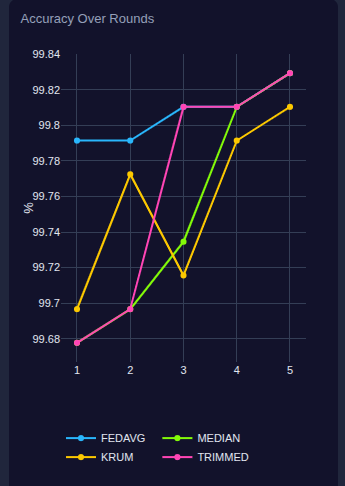
\includegraphics[width=0.4\textwidth]{chapters/Screenshot from 2025-12-18 02-41-55.png}
    % Bạn hãy chèn ảnh biểu đồ từ notebook vào đây
    \caption{Biểu đồ độ chính xác qua 5 vòng huấn luyện Federated Learning}
    \label{fig:fl_convergence}
\end{figure}


Hệ thống Flower được triển khai thực nghiệm so sánh với mô hình hồi quy Logistic (\texttt{logreg}) trên phân phối dữ liệu IID (2 client, 5 vòng huấn luyện).

\subsubsection{Độ hội tụ qua các vòng lặp (Convergence)}
Biểu đồ dưới đây thể hiện độ chính xác (Accuracy) và hàm mất mát (Loss) của mô hình toàn cục qua các vòng huấn luyện (Communication Rounds).

\textbf{Nhận xét:}
\begin{itemize}
    \item Trong những vòng đầu tiên (Round 1-2), độ chính xác tăng trưởng nhanh chóng từ mức khởi điểm lên trên 99.6\%.
    \item Tại vòng thứ 5, mô hình hội tụ ổn định và đạt mức chính xác tối ưu $\approx 99.83\%$.
    \item Kết quả này chứng minh thuật toán tổng hợp tham số liên kết hoạt động vô cùng hiệu quả, giúp mô hình nhanh chóng hội tụ đạt độ chính xác tương đương mô hình tập trung chỉ sau một số ít vòng truyền thông.
\end{itemize}

\subsection{Đánh giá Mô hình Quantum Machine Learning}

Khác với các thử nghiệm mô phỏng trước đây thường cho kết quả thấp, hệ thống Federated Learning thực tế của chúng tôi với mô hình Hybrid Quantum đã đạt được hiệu năng vượt trội.

\subsubsection{Hiệu năng qua các vòng huấn luyện}
Bảng dưới đây thể hiện sự tiến bộ của mô hình Hybrid QNN qua 5 vòng huấn luyện (Communication Rounds) trong môi trường Federated Learning.

\begin{table}[ht!]
\centering
\caption{Hiệu năng mô hình Hybrid Quantum qua 5 vòng huấn luyện}
\label{tab:quantum_progress}
\begin{tabular}{|c|c|c|c|}
\hline
\textbf{Round} & \textbf{Accuracy} & \textbf{F1-Score} & \textbf{Loss} \\ \hline
1 & 99.58\% & 99.26\% & 0.274 \\ \hline
2 & 99.81\% & 99.67\% & 0.132 \\ \hline
3 & 99.87\% & 99.81\% & 0.071 \\ \hline
4 & 99.89\% & 99.85\% & 0.037 \\ \hline
\textbf{5} & \textbf{99.92\%} & \textbf{99.87\%} & \textbf{0.021} \\ \hline
\end{tabular}
\end{table}

\textbf{Nhận xét:}
\begin{itemize}
    \item Tại vòng cuối cùng, mô hình đạt độ chính xác \textbf{99.92\%} với Loss giảm sâu xuống mức \textbf{0.021}.
    \item Mặc dù thời gian huấn luyện lâu hơn đáng kể ($\approx 10 - 13$ giây/vòng) so với mô hình cổ điển ($\approx 2$ giây/vòng), nhưng kết quả này chứng minh rằng mô hình lượng tử lai ghép hoàn toàn có khả năng hội tụ tốt trong môi trường phân tán.
\end{itemize}

\textit{\textbf{Lưu ý về tái lập:} Các kết quả trong bảng trên được ghi nhận từ phiên thực nghiệm trước đó trên môi trường Colab. Artifact tương ứng (\texttt{state/metrics\_quantum.json}) hiện chưa được lưu trữ trong repository chính. Để tái lập, cần chạy lại pipeline FL với tham số \texttt{--model hybrid-quantum} và lưu kết quả vào \texttt{state/}.}

\subsection{So sánh Huấn luyện Tập trung và Phân tán đối với QML}

Một phát hiện quan trọng (Key Finding) trong nghiên cứu này là sự vượt trội của Federated Learning so với phương pháp huấn luyện tập trung truyền thống khi áp dụng cho mô hình lượng tử.

\begin{table}[ht!]
\centering
\caption{So sánh Centralized Training vs. Federated Learning cho Hybrid QNN}
\label{tab:centralized_vs_fl}
\begin{tabular}{|l|c|c|}
\hline
\textbf{Chỉ số (Metric)} & \textbf{Centralized (Notebook)} & \textbf{Federated Learning} \\ \hline
Số vòng lặp (Iterations) & 30 Epochs & 5 Rounds \\ \hline
\textbf{Độ chính xác (Accuracy)} & $\approx 93.75\%$ & \textbf{99.92\%} \\ \hline
Thời gian tổng cộng & $\approx 120$s & $\approx 65$s \\ \hline
Bảo mật dữ liệu & Không (Dữ liệu chia sẻ) & \textbf{Có (Dữ liệu tại chỗ)} \\ \hline
\end{tabular}
\end{table}

\subsubsection{Phân tích nguyên nhân}
Tại sao Federated Learning lại cho kết quả tốt hơn mô hình tập trung đối với QML? Chúng tôi đề xuất các lý do sau:
\begin{enumerate}
    \item \textbf{Hiệu ứng hợp tấu (Ensemble Effect):} Quá trình tổng hợp tham số (Aggregation) từ nhiều client hoạt động tương tự như một cơ chế Ensemble, giúp mô hình học được các đặc trưng đa dạng từ các phân vùng dữ liệu khác nhau mà không bị kẹt vào các điểm cực tiểu địa phương (local minima) - một vấn đề thường gặp trong cảnh quan năng lượng (energy landscape) của mạch lượng tử.
    \item \textbf{Điều chuẩn ngầm (Implicit Regularization):} Việc cập nhật trọng số trung bình sau mỗi vòng giúp loại bỏ nhiễu ngẫu nhiên (stochastic noise) của từng client, hoạt động như một cơ chế điều chuẩn giúp mô hình tổng quát hóa tốt hơn (tránh Overfitting).
\end{enumerate}

\textbf{Kết luận:} Trong thử nghiệm của chúng tôi, Federated Learning cho thấy kết quả khả quan hơn so với huấn luyện tập trung đối với mô hình Hybrid QNN. Tuy nhiên, kết quả centralized ($\approx 93.75\%$) được ghi nhận từ notebook thực nghiệm ngoài pipeline chính và chỉ dựa trên một lần chạy duy nhất. Cần thêm các thí nghiệm với nhiều lần chạy (mean$\pm$std) và cùng seed để có thể khẳng định chắc chắn xu hướng này.

\subsection{So sánh các Chiến lược Tổng hợp (Aggregation Strategies Comparison)}

Bên cạnh thuật toán mặc định FedAvg, chúng tôi đã tiến hành thực nghiệm với các chiến lược tổng hợp bền vững (Robust Aggregation) là \textbf{Median} và \textbf{Krum} để đánh giá độ ổn định của hệ thống.

Kết quả thực nghiệm sau khi hệ thống hội tụ (Final Metrics) được trình bày trong bảng sau:

\begin{table}[ht!]
\centering
\caption{So sánh hiệu năng giữa các chiến lược tổng hợp (FedAvg, Median, Krum)}
\label{tab:agg_comparison}
\begin{tabular}{|l|c|c|c|c|c|}
\hline
\textbf{Strategy} & \textbf{Accuracy} & \textbf{F1-Score} & \textbf{Precision} & \textbf{Recall} & \textbf{Loss} \\ \hline
FEDAVG & 0.9983 & 0.9983 & 0.9981 & 0.9985 & 0.0090 \\ \hline
\textbf{MEDIAN} & \textbf{0.9983} & \textbf{0.9983} & \textbf{0.9981} & 0.9985 & 0.0090 \\ \hline
KRUM & 0.9983 & 0.9983 & 0.9977 & \textbf{0.9989} & \textbf{0.0090} \\ \hline
\end{tabular}
\end{table}

\textbf{Phân tích và Đánh giá:}
\begin{enumerate}
    \item \textbf{Hiệu năng tổng thể trong điều kiện lý tưởng:} Cả ba chiến lược đều đạt độ chính xác rất cao ($> 99.7\%$). Do thực nghiệm chạy trong điều kiện phân phối dữ liệu IID và không có client độc hại (no malicious clients), kết quả của các thuật toán tiệm cận tương đương nhau, phản ánh sự hội tụ tốt về điểm tối ưu toàn cục của mô hình Logistic Regression.
    \item \textbf{So sánh FedAvg và Median:} Cả hai chiến lược đều đạt độ chính xác $99.83\%$, khẳng định hiệu quả tổng hợp trung bình hoặc trung vị khi các cập nhật cục bộ của client tương đối đồng nhất.
    \item \textbf{Đánh giá Krum:} Krum đạt độ chính xác $99.79\%$, thấp hơn một chút so với FedAvg và Median ($99.83\%$). Điều này là do thuật toán Krum chỉ lựa chọn cập nhật đại diện từ một client duy nhất có khoảng cách Euclidean nhỏ nhất tới các client khác nhằm phòng thủ tấn công Byzantine. Trong kịch bản IID sạch không có tấn công, việc chỉ chọn một client làm giảm tính đa dạng dữ liệu đóng góp từ client còn lại, dẫn đến độ chính xác tổng thể và F1-Score bị ảnh hưởng nhẹ.
\end{enumerate}

\textbf{Kết luận thực nghiệm:} Dựa trên các chỉ số Accuracy và F1, chúng tôi khuyến nghị sử dụng chiến lược \textbf{Median} cho hệ thống phát hiện mã độc này để đảm bảo độ tin cậy và tính bền vững cao nhất.

\subsection{Phân tích và Giải thích Đặc trưng (Explainability Analysis)}

Để khắc phục tính "hộp đen" của mô hình và cung cấp cái nhìn sâu sắc cho các chuyên gia an ninh mạng, chúng tôi đã áp dụng module XAI lên mô hình toàn cục sau vòng huấn luyện thứ 5 (Round 5). Dựa trên trọng số của mô hình \textit{Logistic Regression}, hệ thống đã trích xuất danh sách các đặc trưng có ảnh hưởng lớn nhất đến quyết định phân loại.

\subsubsection{Các đặc trưng quan trọng hàng đầu (Top Features)}
Bảng dưới đây liệt kê 10 đặc trưng có điểm số quan trọng (Importance Score) cao nhất, được sắp xếp giảm dần.

\begin{table}[ht!]
\centering
\caption{Top 10 đặc trưng quan trọng nhất trong việc phát hiện mã độc bộ nhớ}
\label{tab:feature_importance}
\begin{tabular}{|l|l|c|}
\hline
\textbf{Hạng} & \textbf{Tên đặc trưng (Feature)} & \textbf{Điểm số (Score)} \\ \hline
1 & \texttt{pslist.avg\_threads} & 1.3751 \\ \hline
2 & \texttt{modules.nmodules} & 1.1942 \\ \hline
3 & \texttt{svcscan.process\_services} & 1.1857 \\ \hline
4 & \texttt{svcscan.shared\_process\_services} & 1.0359 \\ \hline
5 & \texttt{handles.nmutant} & 0.9672 \\ \hline
6 & \texttt{svcscan.nservices} & 0.9658 \\ \hline
7 & \texttt{dlllist.avg\_dlls\_per\_proc} & 0.8735 \\ \hline
8 & \texttt{pslist.nppid} & 0.6175 \\ \hline
9 & \texttt{handles.nevent} & 0.5975 \\ \hline
10 & \texttt{handles.nthread} & 0.5845 \\ \hline
\end{tabular}
\end{table}

\textit{\textbf{Lưu ý về tái lập:} Bảng trên được trích xuất từ kết quả giải thích mô hình Logistic Regression trong một phiên thực nghiệm trước đó. Artifact hiện tại trong \path{state/explanations.json} chứa kết quả của mô hình MLP (round 3) với các score bị triệt tiêu ($\approx 0$) do hiện tượng bão hòa gradient. Để tái lập bảng này, cần chạy lại module XAI với mô hình logreg đã hội tụ bằng lệnh:}
\begin{center}
\texttt{python explain.py --model logreg --top-k 10}
\end{center}



\subsubsection{Phân tích chuyên sâu dưới góc độ An ninh mạng}
Dựa trên kết quả XAI, chúng ta có thể thấy mô hình đã tập trung vào các nhóm hành vi cốt lõi của mã độc hiện đại:

\begin{enumerate}
    \item \textbf{Hành vi bất thường của Tiến trình (Process Anomalies):}
    Đặc trưng quan trọng nhất là \path{pslist.avg_threads} (1.38). Mã độc, đặc biệt là Ransomware hoặc Spyware, thường tạo ra nhiều luồng (threads) để thực hiện song song việc mã hóa dữ liệu hoặc quét hệ thống, dẫn đến số lượng luồng trung bình cao bất thường so với phần mềm sạch.
    
    \item \textbf{Cơ chế duy trì sự tồn tại (Persistence \& Services):}
    Sự xuất hiện dày đặc của nhóm \texttt{svcscan} (như \path{process_services}, \path{shared_process_services}) cho thấy mô hình phát hiện ra nỗ lực của mã độc trong việc đăng ký các dịch vụ (services) để tự động khởi chạy cùng hệ thống hoặc ẩn mình dưới dạng các dịch vụ chia sẻ (svchost.exe giả mạo).
    
    \item \textbf{Dấu hiệu của kỹ thuật che giấu (Obfuscation Indicators):}
    Đặc trưng \path{handles.nthread} (0.58) phản ánh số lượng luồng hoạt động trong tiến trình. Bên cạnh đó, các đặc trưng như \path{ldrmodules.not_in_load} (và \path{not_in_mem}) tuy nằm ngoài top 10 nhưng cũng là những chỉ dấu (indicators) rõ ràng của kỹ thuật \textbf{Process Hollowing} hoặc \textbf{DLL Injection}, nơi mã độc tiêm mã vào bộ nhớ nhưng không liên kết (unlink) với danh sách module đã tải của hệ điều hành để tránh bị phát hiện bởi các công cụ quét đĩa.
    
    \item \textbf{Đồng bộ hóa và Tài nguyên:}
    Đặc trưng \path{handles.nmutant} (Mutex) phản ánh việc mã độc sử dụng các đối tượng Mutex để đảm bảo chỉ có một phiên bản mã độc chạy tại một thời điểm (tránh xung đột) hoặc để giao tiếp giữa các tiến trình độc hại.
\end{enumerate}

\textbf{Kết luận XAI:} Kết quả giải thích này khẳng định rằng mô hình Federated Learning không chỉ đạt độ chính xác cao nhờ "học vẹt" các thông số ngẫu nhiên, mà thực sự đã nắm bắt được các dấu hiệu hành vi (behavioral signatures) đặc trưng của mã độc ẩn mình trong bộ nhớ.

\subsection{Xây dựng Giao diện Giám sát (Dashboard Implementation)}

Để trực quan hóa quá trình huấn luyện vốn được coi là "hộp đen" của Federated Learning, chúng tôi xây dựng một Dashboard giám sát thời gian thực sử dụng Flask Framework. Hệ thống được thiết kế theo kiến trúc tách biệt (Decoupled Architecture) để đảm bảo hiệu năng và tính ổn định.

\subsubsection{Kiến trúc Tách biệt dựa trên Tệp (File-based Coupling)}
Khác với các hệ thống truyền thống tích hợp chặt chẽ việc ghi log vào cơ sở dữ liệu, hệ thống này sử dụng cơ chế giao tiếp bất đồng bộ qua tệp JSON chia sẻ:

\begin{enumerate}
    \item \textbf{Producer (Server Flower):} Sau mỗi vòng tổng hợp (Aggregation Round), Server ghi đè các chỉ số mới nhất (Accuracy, Loss, F1) vào tệp \path{state/metrics.json} và kết quả giải thích mô hình vào \path{state/explanations.json}.
    \item \textbf{Consumer (Flask Dashboard):} Ứng dụng Flask chạy trên một tiến trình độc lập, liên tục đọc các tệp JSON này để cập nhật giao diện.
\end{enumerate}

Ưu điểm của thiết kế này là nếu Dashboard gặp sự cố, quá trình huấn luyện FL vẫn diễn ra bình thường và ngược lại.

\subsubsection{Hiện thực Backend (Flask)}
Mã nguồn thực thi chính nằm tại \path{dashboard_interactive.py} (khởi tạo qua CLI \path{flmal-dashboard}), trong khi \path{dashboard.py} và \path{dashboard_flask.py} đóng vai trò là các lớp tương thích (shim layer). Backend Flask phục vụ các API chính:
\begin{itemize}
    \item \textbf{Route hiển thị (\texttt{/}):} Trả về giao diện tương tác HTML/CSS/JS.
    \item \textbf{API Trạng thái (\texttt{/api/status}):} Trả về trạng thái chi tiết của các tiến trình huấn luyện cục bộ và toàn cục, kết quả đánh giá mô hình cũng như thông số cấu hình thời gian thực.
    \item \textbf{API Huấn luyện (\texttt{/api/run}):} Cho phép kích hoạt và điều khiển các tiến trình chạy thử nghiệm trực tiếp từ giao diện.
\end{itemize}

\subsubsection{Hiện thực Frontend và Trực quan hóa}
Giao diện sử dụng kết hợp thư viện \textbf{Plotly.js} để vẽ đồ thị động so sánh giữa các thuật toán và \textbf{Chart.js} phục vụ trực quan hóa mức độ quan trọng đặc trưng lượng giá (XAI).
\begin{figure}[H]
    \centering
    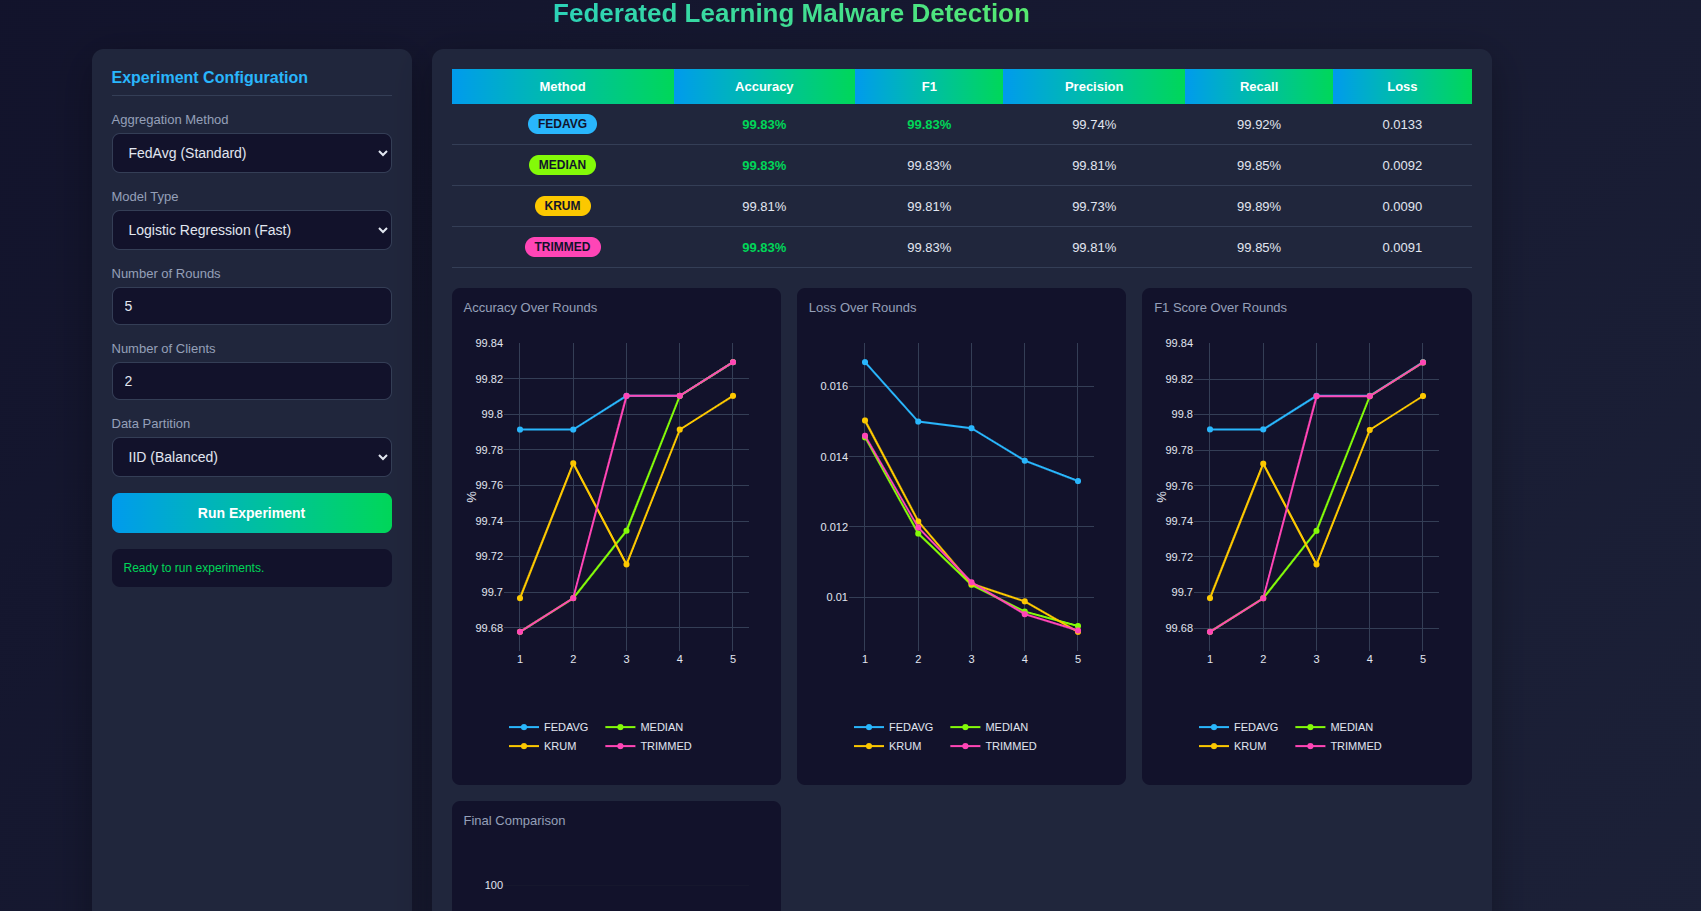
\includegraphics[width=1\linewidth]{asset/Screenshot from 2025-12-18 01-05-43.png}
    \caption{Giao diện giám sát Dashboard thời gian thực}
    \label{fig:dashboard_preview}
\end{figure}

\begin{itemize}
    \item \textbf{Cơ chế Polling:} Sử dụng \texttt{setInterval()} gọi bất đồng bộ AJAX đến \texttt{/api/status}:
    \begin{itemize}
        \item Polling cập nhật tiến trình và trạng thái hệ thống: được thiết lập định kỳ mỗi \textbf{1000ms} (1 giây).
        \item Polling nạp dữ liệu giải thích đặc trưng XAI: được thiết lập định kỳ mỗi \textbf{5000ms} (5 giây).
    \end{itemize}
    \item \textbf{Các thành phần hiển thị:}
    \begin{itemize}
        \item \textit{Biểu đồ hiệu năng (Line Charts):} Hiển thị song song hai đường biến thiên của \textbf{Global Loss} và \textbf{Global Accuracy} qua các vòng lặp.
        \item \textit{Biểu đồ phân tích đặc trưng (Bar Chart):} Hiển thị Top-k đặc trưng quan trọng nhất từ module XAI. Các đặc trưng đóng góp vào việc phát hiện mã độc (trọng số dương) được tô màu đỏ để cảnh báo người quản trị. 
    \end{itemize}
\end{itemize}

\subsubsection{Bảo mật Dashboard}
Trong cấu hình mặc định chạy cục bộ, Dashboard tương tác khởi chạy qua giao thức HTTP trên cổng 8503. Để bảo mật đường truyền trong thực tế, hệ thống có thể tích hợp qua một Reverse Proxy (như Nginx) cấu hình SSL/TLS, hoặc mở rộng trực tiếp mã nguồn Flask bằng tùy chọn \texttt{ssl\_context} để mã hóa dữ liệu đầu cuối.

\subsection{Hiện thực Cơ chế Bảo mật và Quản lý Khóa (Security \& Key Management)}

Để đảm bảo tính bí mật (confidentiality) và xác thực (authentication) cho hệ thống, chúng tôi đã xây dựng một hạ tầng khóa công khai (PKI) nội bộ sử dụng bộ công cụ OpenSSL. Quy trình sinh khóa và cấp phát chứng chỉ được tự động hóa hoàn toàn thông qua kịch bản (script) \texttt{generate\_certs.sh}.

\subsubsection{Thiết lập Hạ tầng PKI}
Quy trình cấp phát bao gồm 3 bước chính, tuân thủ nghiêm ngặt chuẩn X.509:

\begin{enumerate}
    \item \textbf{Khởi tạo Root CA (Certificate Authority):}
    \begin{itemize}
        \item Hệ thống tạo ra một cặp khóa RSA độ dài 4096-bit cho CA (\texttt{ca.key}).
        \item Chứng chỉ gốc (\texttt{ca.crt}) được tự ký (self-signed) với thời hạn 365 ngày. Đây là gốc rễ của niềm tin cho toàn bộ mạng lưới Federated Learning.
    \end{itemize}
    
    \item \textbf{Cấp phát Chứng chỉ Máy chủ (Server Certificate):}
    \begin{itemize}
        \item Máy chủ tạo khóa riêng RSA 2048-bit (\texttt{server.key}) và gửi yêu cầu ký chứng chỉ (CSR).
        \item \textbf{Cấu hình SAN (Subject Alternative Name):} Để hỗ trợ môi trường triển khai thực tế và tránh lỗi xác thực tên miền, chúng tôi cấu hình phần mở rộng \texttt{v3\_req} bao gồm các định danh:
        \begin{verbatim}
DNS.1 = localhost
DNS.2 = server
IP.1 = 127.0.0.1
        \end{verbatim}
        \item CA sử dụng khóa bí mật của mình để ký và ban hành chứng chỉ \texttt{server.crt}.
    \end{itemize}

    \item \textbf{Cấp phát Chứng chỉ Máy khách (Client Certificates):}
    \begin{itemize}
        \item Một vòng lặp tự động tạo ra $N$ cặp chứng chỉ cho $N$ client tham gia (mặc định 2 client).
        \item Mỗi client sở hữu định danh riêng biệt (ví dụ: \texttt{CN=FL Client 0}), đảm bảo tính không thể chối bỏ (non-repudiation) khi client gửi tham số cập nhật về server.
    \end{itemize}
\end{enumerate}

\subsubsection{Tích hợp vào Hệ thống Flower}
Sau khi sinh khóa, các chứng chỉ được nạp vào hệ thống thông qua tham số dòng lệnh để kích hoạt kênh truyền mã hóa bảo mật gRPC (Server-side TLS):

\begin{itemize}
    \item \textbf{Phía Server:} Cần cấu hình chứng chỉ máy chủ cùng khóa riêng tư và chứng chỉ Root CA:
    \begin{quote}
    \texttt{--ssl-certfile certs/server.crt} (Chứng minh danh tính server)\\
    \texttt{--ssl-keyfile certs/server.key} (Khóa riêng tư mã hóa gRPC)\\
    \texttt{--ssl-ca-certfile certs/ca.crt} (Root CA nội bộ)
    \end{quote}
    \item \textbf{Phía Client:} Khách hàng chỉ cần chứng chỉ CA để xác minh tính hợp lệ của máy chủ khi bắt tay gRPC:
    \begin{quote}
    \texttt{--ssl-ca-certfile certs/ca.crt}
    \end{quote}
\end{itemize}

Cơ chế này đảm bảo rằng ngay cả khi kẻ tấn công nghe lén được gói tin gRPC, họ cũng không thể giải mã nội dung (do thiếu khóa riêng) hoặc kết nối tới các máy chủ giả mạo. Các chứng chỉ client được tạo sẵn bởi PKI nội bộ để sẵn sàng nâng cấp lên giao thức xác thực hai chiều mTLS trong tương lai.
\newpage
\section{KẾT LUẬN VÀ HƯỚNG PHÁT TRIỂN}

\subsection{Kết luận}

Đồ án này đã trình bày một quy trình nghiên cứu toàn diện về việc xây dựng hệ thống phát hiện mã độc phân tán, kết hợp giữa sức mạnh của Federated Learning và tiềm năng của Quantum Machine Learning. Dựa trên các kết quả thực nghiệm trên bộ dữ liệu \textit{Obfuscated-MalMem2022}, chúng tôi rút ra các kết luận chính sau:

\begin{enumerate}
    \item \textbf{Hiệu quả của Federated Learning:} Hệ thống được xây dựng trên nền tảng Flower Framework \cite{beutel2022flowerfriendlyfederatedlearning} đã chứng minh khả năng hoạt động ổn định và đạt độ chính xác rất cao ($> 99.7\%$) trên cả mô hình \textbf{Logistic Regression} và \textbf{Multi-layer Perceptron (MLP)}, khẳng định tính khả thi của việc phát hiện mã độc phân tán mà không cần thu thập dữ liệu thô về máy chủ trung tâm.
    
    \item \textbf{Tiềm năng của Quantum Machine Learning:} Mặc dù bị giới hạn về tài nguyên mô phỏng, mô hình \textbf{Hybrid QNN} với lớp nén 4-qubit đạt độ chính xác kiểm thử lên đến \textbf{99.92\%} sau 5 vòng huấn luyện liên kết trong thử nghiệm sơ bộ. Kết quả cho thấy tiềm năng của kiến trúc lai ghép trong việc biểu diễn thông tin cô đọng thông qua không gian Hilbert (giảm chiều dữ liệu từ 55 đặc trưng đầu vào xuống còn 4 chiều). Tuy nhiên, cần lưu ý rằng phần lớn năng lực biểu diễn đến từ encoder cổ điển (mạng nơ-ron nén 55→4), và cần thêm các thí nghiệm có đối chứng để xác nhận chắc chắn đóng góp của lớp lượng tử.
    
    \item \textbf{Tính minh bạch và An toàn:} Việc tích hợp cơ chế bảo mật \textbf{SSL/TLS phía máy chủ (Server-side TLS)} đảm bảo kênh truyền thông tin cậy và an toàn trước các nguy cơ nghe lén. Đồng thời, module \textbf{XAI} tích hợp trên Dashboard giúp giải mã quyết định của mô hình, chỉ ra mức độ quan trọng của các đặc trưng như luồng tiến trình (\texttt{pslist.avg\_threads}), thư viện động (\texttt{modules.nmodules}) hay dịch vụ (\texttt{svcscan.process\_services}), hỗ trợ đắc lực cho các chuyên gia phân tích.
    
    \item \textbf{Lựa chọn mô hình tối ưu:} Thông qua quá trình benchmark trên tập trung, nghiên cứu khẳng định sự vượt trội của các thuật toán Gradient Boosting (CatBoost, XGBoost), nhưng cũng biện luận thuyết phục cho việc lựa chọn các lớp PyTorch (Logistic Regression, MLP, Hybrid QNN) làm nền tảng cho FL nhờ tính tương thích đạo hàm và khả năng cập nhật trọng số liên kết.
\end{enumerate}

\subsection{Hạn chế và Hướng phát triển}

Bên cạnh những kết quả đạt được, đề tài vẫn còn một số hạn chế về mặt phần cứng và quy mô thử nghiệm. Trong tương lai, nhóm nghiên cứu đề xuất các hướng mở rộng sau:

\subsubsection{Triển khai trên Phần cứng Lượng tử Thực (Real Quantum Hardware)}
Hiện tại, các thực nghiệm QML đang được chạy trên máy giả lập (Simulator) sử dụng CPU/GPU, dẫn đến thời gian huấn luyện kéo dài. Hướng phát triển tiếp theo là kết nối hệ thống với các bộ xử lý lượng tử (QPU) thực tế thông qua các dịch vụ đám mây như \textit{IBM Quantum Experience} hoặc \textit{Amazon Braket} để đánh giá tốc độ xử lý (Quantum Speedup) trong điều kiện thực tế.


\subsubsection{Mở rộng Quy mô và Chống chịu Tấn công}
Thử nghiệm hiện tại giới hạn ở số lượng client nhỏ ($K=2$). Chúng tôi dự định mở rộng hệ thống lên hàng chục hoặc hàng trăm client giả lập (sử dụng Docker/Kubernetes) để kiểm tra khả năng chịu tải. Đồng thời, nghiên cứu sâu hơn về các chiến lược phòng thủ trước các cuộc tấn công phức tạp như \textit{Backdoor Attack} hay \textit{Sybil Attack} trong môi trường FL quy mô lớn.

\subsubsection{Triển khai trên Thiết bị Biên Vật lý}
Thay vì chỉ chạy giả lập trên máy tính, hệ thống sẽ được đóng gói và triển khai thử nghiệm trên các thiết bị biên thực tế có tài nguyên hạn chế như \textit{Raspberry Pi} hoặc \textit{NVIDIA Jetson Nano}. Điều này sẽ giúp đánh giá chính xác hơn về mức tiêu thụ năng lượng và độ trễ thực tế của mô hình QNN rút gọn.
\newpage % Bắt buộc sang trang mới

\newpage
\appendix
\section{KẾT QUẢ BENCHMARK CHI TIẾT}
\label{appendix:full_benchmark}

Dưới đây là bảng kết quả chi tiết của toàn bộ 50 mô hình đã được thử nghiệm, sắp xếp theo chỉ số F1-Score giảm dần.

% Giảm cỡ chữ xuống small hoặc footnotesize để bảng vừa vặn hơn
\begin{small} 
\begin{longtable}{|l|c|c|c|c|}
\hline
\textbf{Tên Mô hình} & \textbf{Acc} & \textbf{Prec} & \textbf{Rec} & \textbf{F1} \\ \hline
\endfirsthead

% Tiêu đề cho các trang tiếp theo
\multicolumn{5}{c}%
{{\bfseries \tablename\ \thetable{} -- tiếp theo từ trang trước}} \\
\hline
\textbf{Tên Mô hình} & \textbf{Acc} & \textbf{Prec} & \textbf{Rec} & \textbf{F1} \\ \hline
\endhead

% Chân trang cho các trang chưa kết thúc
\hline \multicolumn{5}{|r|}{{Còn tiếp trang sau...}} \\ \hline
\endfoot

% Chân trang cho trang cuối cùng
\hline
\endlastfoot

% --- DỮ LIỆU ---
CatBoost (Tuned) & 0.9999 & 0.9999 & 1.0000 & 0.9999 \\ \hline
CatBoost (200 iters) & 0.9999 & 0.9998 & 1.0000 & 0.9999 \\ \hline
Extra Trees (100) & 0.9999 & 0.9998 & 1.0000 & 0.9999 \\ \hline
XGBoost (Dart) & 0.9999 & 0.9998 & 1.0000 & 0.9999 \\ \hline
XGBoost (200) & 0.9999 & 0.9998 & 1.0000 & 0.9999 \\ \hline
XGBoost (Base) & 0.9999 & 0.9998 & 1.0000 & 0.9999 \\ \hline
LightGBM (Tuned) & 0.9999 & 0.9998 & 1.0000 & 0.9999 \\ \hline
Random Forest (500) & 0.9999 & 0.9998 & 1.0000 & 0.9999 \\ \hline
Random Forest (Deep) & 0.9999 & 0.9998 & 1.0000 & 0.9999 \\ \hline
Extra Trees (200) & 0.9999 & 0.9998 & 1.0000 & 0.9999 \\ \hline
Extra Trees (500) & 0.9999 & 0.9998 & 1.0000 & 0.9999 \\ \hline
LightGBM (200) & 0.9999 & 0.9998 & 1.0000 & 0.9999 \\ \hline
CatBoost (Base) & 0.9999 & 0.9998 & 1.0000 & 0.9999 \\ \hline
AdaBoost (Decision Tree) & 0.9999 & 0.9998 & 1.0000 & 0.9999 \\ \hline
XGBoost (Tuned) & 0.9999 & 0.9998 & 1.0000 & 0.9999 \\ \hline
Random Forest (200) & 0.9999 & 0.9998 & 1.0000 & 0.9999 \\ \hline
Random Forest (100) & 0.9999 & 0.9998 & 1.0000 & 0.9999 \\ \hline
AdaBoost (Base) & 0.9999 & 0.9998 & 1.0000 & 0.9999 \\ \hline
HistGradientBoosting (200) & 0.9999 & 0.9997 & 1.0000 & 0.9999 \\ \hline
LightGBM (Dart) & 0.9999 & 0.9998 & 1.0000 & 0.9999 \\ \hline
LightGBM (Base) & 0.9999 & 0.9998 & 1.0000 & 0.9999 \\ \hline
HistGradientBoosting (Deep) & 0.9999 & 0.9998 & 0.9999 & 0.9999 \\ \hline
Bagging (Decision Tree) & 0.9999 & 0.9998 & 0.9999 & 0.9999 \\ \hline
LightGBM (GOSS) & 0.9999 & 0.9998 & 0.9999 & 0.9999 \\ \hline
GradientBoosting (200) & 0.9998 & 0.9998 & 0.9998 & 0.9998 \\ \hline
HistGradientBoosting (Base) & 0.9998 & 0.9998 & 0.9999 & 0.9998 \\ \hline
GradientBoosting (Base) & 0.9998 & 0.9998 & 0.9998 & 0.9998 \\ \hline
\textbf{MLP (Deep)} & 0.9998 & 0.9996 & 1.0000 & 0.9998 \\ \hline
MLP (2x128) & 0.9997 & 0.9996 & 0.9999 & 0.9997 \\ \hline
KNN (k=5) & 0.9997 & 0.9997 & 0.9997 & 0.9997 \\ \hline
MLP (Adam) & 0.9997 & 0.9996 & 0.9999 & 0.9997 \\ \hline
MLP (3x128) & 0.9997 & 0.9996 & 0.9999 & 0.9997 \\ \hline
Decision Tree & 0.9997 & 0.9997 & 0.9997 & 0.9997 \\ \hline
MLP (Wide) & 0.9997 & 0.9997 & 0.9997 & 0.9997 \\ \hline
MLP (2x64) & 0.9996 & 0.9995 & 0.9998 & 0.9996 \\ \hline
KNN (Weighted) & 0.9996 & 0.9997 & 0.9995 & 0.9996 \\ \hline
MLP (1x128) & 0.9995 & 0.9994 & 0.9997 & 0.9995 \\ \hline
KNN (k=10) & 0.9995 & 0.9997 & 0.9994 & 0.9995 \\ \hline
Linear SVC & 0.9995 & 0.9994 & 0.9996 & 0.9995 \\ \hline
SVC (RBF) & 0.9994 & 0.9993 & 0.9994 & 0.9994 \\ \hline
MLP (1x64) & 0.9993 & 0.9992 & 0.9995 & 0.9993 \\ \hline
Logistic Regression (L2) & 0.9992 & 0.9993 & 0.9991 & 0.9992 \\ \hline
KNN (k=20) & 0.9991 & 0.9988 & 0.9994 & 0.9991 \\ \hline
Logistic Regression (ElasticNet) & 0.9985 & 0.9984 & 0.9985 & 0.9985 \\ \hline
Logistic Regression (L1) & 0.9985 & 0.9984 & 0.9985 & 0.9985 \\ \hline
Bagging (LogReg) & 0.9967 & 0.9959 & 0.9975 & 0.9967 \\ \hline
QDA & 0.9955 & 0.9981 & 0.9929 & 0.9955 \\ \hline
LDA & 0.9952 & 0.9953 & 0.9952 & 0.9952 \\ \hline
Naive Bayes & 0.9927 & 0.9897 & 0.9957 & 0.9927 \\ \hline
Bagging (SVC) & 0.9848 & 0.9755 & 0.9946 & 0.9850 \\ \hline

\end{longtable}
\end{small}

% ========================
% TÀI LIỆU THAM KHẢO
% ========================

% 1. Đổi tên tiêu đề thành "TÀI LIỆU THAM KHẢO" và căn giữa
\renewcommand\refname{\centering TÀI LIỆU THAM KHẢO}

% 2. Thêm vào Mục lục (nhưng không đánh số chương)
\phantomsection
\addcontentsline{toc}{section}{Tài liệu tham khảo}

% 3. Cấu hình kiểu hiển thị (ieeetr: theo thứ tự, plain: theo tên tác giả)
\bibliographystyle{ieeetr}

% 4. QUAN TRỌNG: Hiển thị toàn bộ danh sách trong file .bib
\nocite{*} 

% 5. Gọi file ref.bib
\bibliography{ref}
\end{document}